%%% Exemplo de utilização da classe ITA
%%%
%%%   por        Fábio Fagundes Silveira   -  ffs [at] ita [dot] br
%%%              Benedito C. O. Maciel     -  bcmaciel [at] ita [dot] br
%%%              Giovani Volnei Meinertz   -  giovani [at] ita [dot] br
%%%    	         Hudson Alberto Bode       -  bode [at] ita [dot]br
%%%    	         P. I. Braga de Queiroz    -  pi [at] ita [dot] br
%%%    	         Jorge A. B. Gripp         -  gripp [at] ita [dot] br
%%%    	         Juliano Monte-Mor         -  jamontemor [at] yahoo [dot] com [dot] br
%%%    	         Tarcisio A. B. Gripp      -  tarcisio.gripp [at] gmail [dot] com
%%%    	         
%%%
%%%  IMPORTANTE: O texto contido neste exemplo nao significa absolutamente nada.  :-)
%%%              O intuito aqui eh demonstrar os comandos criados na classe e suas
%%%              respectivas utilizacoes.
%%%
%%%  Tese.tex  2016-08-25
%%%  $HeadURL: http://www.apgita.org.br/apgita/teses-e-latex.php $
%%%
%%% ITALUS
%%% Instituto Tecnológico de Aeronáutica --- ITA, Sao Jose dos Campos, Brasil
%%%                   http://groups.yahoo.com/group/italus/
%%% Discussion list: italus {at} yahoogroups.com
%%%
%++++++++++++++++++++++++++++++++++++++++++++++++++++++++++++++++++++++++++++++
% Para alterar o TIPO DE DOCUMENTO, preencher a linha abaixo \documentclass[?]{?}
%   \documentclass[tg]{ita}			= Trabalho de Graduacao
%   \documentclass[tgfem]{ita}	= Para Engenheiras
%                   msc     		= Dissertacao de Mestrado
%   				mscfem   		= Para Mestras
%   				dsc      		= Tese de Doutorado
%   				dscfem   		= Para Doutoras
%   				quali    		= Exame de Qualificacao
%   				qualifem 		= Exame de Qualificacao para Doutoras
% Para 'Draft Version'/'Versao Preliminar' com data no rodape, adicionar 'dv':
%   \documentclass[dsc, dv]{ita} 
% Para trabalhos em Inglês, adicionar 'eng':
%   \documentclass[dsc, eng]{ita}
%		\documentclass[dsc, eng, dv]{ita}
%++++++++++++++++++++++++++++++++++++++++++++++++++++++++++++++++++++++++++++++
\documentclass[dv, a4paper, tg]{ita}    % ITA.cls based on standard book.cls 
% Quando alterar a classe, por exemplo de [msc] para [msc, eng]) rode mais uma vez o botão BUILD OUTPUT caso haja erro
\usepackage{ae}
\usepackage{graphicx}
\usepackage{epsfig}
\usepackage{amsmath}
\usepackage{amssymb} 
\usepackage{subcaption}
\usepackage{multirow}
\usepackage{float}

%++++++++++++++++++++++++++++++++++++++++++++++++++++++++++++++++++++++++++++++
% Espaçamento padrão de todo o documento
%++++++++++++++++++++++++++++++++++++++++++++++++++++++++++++++++++++++++++++++
\onehalfspacing

%singlespacing Para um espaçamento simples
%onehalfspacing Para um espaçamento de 1,5
%doublespacing Para um espaçamento duplo

%++++++++++++++++++++++++++++++++++++++++++++++++++++++++++++++++++++++++++++++
% Identificacoes (se o trabalho for em inglês, insira os dados em inglês)
% Para entradas abreviadas de Professora (Profa.) em português escreva: Prof$^\textnormal{a}$.
%++++++++++++++++++++++++++++++++++++++++++++++++++++++++++++++++++++++++++++++
\course{Engenharia Aeroespacial} % Programa de PG ou Curso de Graduação
% \area{Sistemas Aeroespaciais e Mecatrônica} % Área de concentração na PG (Não utilizado no caso de TG)

% Autor do trabalho: {Nome}{Sobrenome}
\authorgender{masc}         % masc ou fem
\author{Henrique}{Silva Simplicio}
\itaauthoraddress{Rua H8B, 234}{12.228-461}{São José dos Campos--SP}

% Titulo da Tese/Dissertação
\title{Implementação do método de colocação direta para otimização de trajetória usando o software MATLAB}

% Orientador
\advisorgender{masc}        % masc ou fem
\advisor{Prof.~Dr.}{Mauricio Andrés Varela Morales}{ITA}

% Coorientador (Caso não haja coorientador, colocar ambas as variáveis \coadvisorgender e \coadvisor comentadas, com um % na frente)
\coadvisorgender{masc}		% masc ou fem
\coadvisor{Prof.~Dr.}{Flávio Luiz Cardoso Ribeiro}{ITA}

% Pró-reitor da Pós-graduação
% \bossgender{masc}           % masc ou fem
% \boss{Prof.~Dr.}{John von Neumann}

%Coordenador do curso no caso de TG
\bosscoursegender{fem}     % masc ou fem
\bosscourse{Profa.~Dra.}{Maisa de Oliveira Terra}

% Palavras-Chaves informadas pela Biblioteca -> utilizada na CIP
% \kwcip{¿}
% \kwcip{¿}
% \kwcip{¿}

% Membros da banca examinadora
\examiner{Prof. Dr.}{¿}{Presidente}{ITA}
\examiner{Prof. Dr.}{¿}{}{UXXX}

% Data da defesa (mês em maiúsculo, se trabalho em inglês, e minúsculo se trabalho em português) 
\date{¿¿}{novembro}{2024}

% Número CDU - (somente para TG)
\cdu{¿¿¿.¿¿}

% Glossario
\makeglossary
\frontmatter

\begin{document}
% Folha de Rosto e Capa para o caso do TG
\maketitle

% Dedicatoria: Nao esqueca essa secao  ... :-)
\begin{itadedication}
Àqueles que sempre me apoiaram e acreditaram em mim, principalmente minha mãe e minha parceira de vida.
\end{itadedication}

% Agradecimentos
\begin{itathanks}
% Primeiramente, gostaria de agradecer ao Dr. Donald E. Knuth, por ter desenvolvido o \TeX.

% Ao Dr. Leslie Lamport, por ter criado o \LaTeX, facilitando muito a utilização do \TeX, e assim, eu não ter que usar o Word.

% Ao Prof. Dr. Meu Orientador, pela orientação e confiança depositada na realização deste trabalho.

% Ao Dr. Nelson D'Ávilla, por emprestar seu nome a essa importante via de trânsito na cidade de São José dos Campos.

% Ah, já estava esquecendo... agradeço também, mais uma vez ao \TeX, por ele não possuir vírus de macro :-)

\end{itathanks}

% Epígrafe
\thispagestyle{empty}
\ifhyperref\pdfbookmark[0]{\nameepigraphe}{epigrafe}\fi
\begin{flushright}
\begin{spacing}{1}
\mbox{}\vfill
{\sffamily\itshape
``Agir conforme aquilo que se fala, alinhar discurso e prática,\\
além de ser uma postura ética, é um sinal de autenticidade.''\\}
--- \textsc{Mario Sergio Cortella}
\end{spacing}
\end{flushright}

% Resumo
\begin{abstract}
\noindent
Este trabalho apresenta o desenvolvimento de uma biblioteca em MATLAB para solução de problemas de otimização de trajetória utilizando o método de colocação direta trapezoidal. A biblioteca visa simplificar a resolução deste tipo de problema, permitindo que o usuário concentre-se apenas na modelagem, sem necessidade de implementar a lógica matemática da solução numérica. A implementação é validada através de três casos de teste: um problema de movimento unidimensional simples, o problema clássico da braquistócrona e um problema de otimização de trajetória de subida de uma aeronave eVTOL. Os resultados obtidos são comparados com soluções analíticas, quando disponíveis, e com resultados da literatura utilizando outros softwares de otimização. O trabalho contribui para a área de controle ótimo ao disponibilizar uma ferramenta que facilita a implementação de soluções numéricas para problemas de otimização de trajetória, sendo particularmente útil para aplicações em engenharia aeroespacial e áreas correlatas.
\end{abstract}

% Abstract
\begin{englishabstract}
\noindent
This work presents the development of a MATLAB library for solving trajectory optimization problems using the trapezoidal direct collocation method. The library aims to simplify the resolution of such problems, allowing users to focus solely on modeling without the need to implement the mathematical logic of the numerical solution. The implementation is validated through three test cases: a simple one-dimensional motion problem, the classic brachistochrone problem, and an eVTOL aircraft climb trajectory optimization problem. The obtained results are compared with analytical solutions, when available, and with results from the literature using other optimization software, demonstrating the effectiveness of the developed library. The work contributes to the field of optimal control by providing a tool that facilitates the implementation of numerical solutions for trajectory optimization problems, being particularly useful for aerospace engineering applications and related fields.
\end{englishabstract}

% Lista de figuras
\listoffigures %opcional

% Lista de tabelas
% \listoftables %opcional

% Lista de abreviaturas
% \listofabbreviations
% \begin{longtable}{ll}
% CTq & computed torque \\
% DC & direct current \\
% EAR & Equação Algébrica de Riccati \\
% GDL & graus de liberdade \\
% ISR & interrupção de serviço e rotina \\
% LMI & linear matrices inequalities \\
% MIMO & multiple input multiple output \\
% PD & proporcional derivativo \\
% PID & proporcional integrativo derivativo \\
% PTP & point to point \\
% UARMII & Underactuated Robot Manipulator II \\
% VSC & variable structure control \\

\end{longtable}

 %opcional

% Lista de simbolos
% \listofsymbols
% \begin{longtable}{ll}
% $a$ & Distância\\
% $\textbf{a}$ & Vetor de distâncias\\
% $\textbf{e}_{j}$ & Vetor unitário de dimensão $n$ e com o $j$-ésimo componente igual a $1$ \\
% $\textbf{K}$ & Matriz de rigidez\\
% $m_1$ & Massa do cumpim\\
% $\delta_{k-k_f}$ & Delta de Kronecker no instante $k_f$\\

\end{longtable}

 %opcional

% Sumario
\tableofcontents

\mainmatter
% Os capitulos comecam aqui

\chapter{Introdução}
\label{cap:introdução}
\section{Motivação}
\label{sec:motivação}

\textcolor{red}{[Não esquecer de inserir motivação aqui]}


\section{Objetivo}
\label{sec:objetivo}

Este trabalho tem como objetivo a implementação de uma biblioteca no MATLAB, que permita a solução de problemas de otimização de trajetória utilizando um método de colocação direta, mais especificamente a colocação trapezoidal. Inspirando-se nos softwares PSOPT \cite{becerra_psopt_2022} e OptimTraj \cite{kelly_optimtraj_2022}, tal biblioteca deverá simplificar a resolução de problemas do tipo, de modo que o usuário deverá apenas modelizar o problema e entrar com os parâmetros necessários por meio de uma interface de dados. Assim, não haverá necessidade de implementar a lógica matemática por trás da solução numérica para obtenção dos resultados pertinentes.


\section{Revisão Bibliográfica}
\label{sec:rev-bibliografica}

Esta seção apresenta uma revisão histórica da otimização de trajetórias, com foco especial na modelagem do problema como um Problema de Controle Ótimo (PCO) e nas técnicas de solução, tanto analíticas quanto numéricas, que culminam na proposta de implementação de métodos de colocação direta usando o software MATLAB.

% Origens e Fundamentos

Iniciamos com as origens da otimização de trajetórias e a modelagem inicial do problema como um PCO. O estudo da otimização de trajetórias tem início com o problema da braquistócrona: encontrar a curva sob a qual uma partícula, sujeita a um campo gravitacional constante, sem atrito e com velocidade inicial nula, leva o menor tempo para se deslocar entre dois pontos \cite{sussmann_300_1997}. Dentre as soluções propostas, a mais famosa usava o Cálculo Variacional.

Por sua vez, o Controle Ótimo tem sua origem ligada ao desenvolvimento do Cálculo Variacional, uma vez que o objetivo do primeiro é minimizar (ou maximizar) uma função objetivo, o que, por sua vez, é o tema estudado pelo segundo. Isaac Newton, Johann Bernoulli, Leonhard Euler e Ludovico Lagrange são alguns importantes nomes que inicialmente contribuíram para o desenvolvimento do Controle Ótimo \cite{becerra_optimal_2008}. Como resultados importantes obtidos no desenvolvimento da teoria, podem-se citar a programação dinâmica \cite{bellman_dynamic_2010}, o princípio mínimo de Pontryagin \cite{pontryagin_mathematical_1987} e a formulação do regulador quadrático linear (\textit{Linear-quadratic Regulator}, LQR) e do filtro de Kalman \cite{kalman_contributions_1960, kalman_new_1960}.

% Soluções Analíticas

Existem diversas excelentes fontes que desenvolvem a teoria do Controle Ótimo, formulando diferentes tipos de problemas e suas soluções \cite{betts_practical_2010, kirk_optimal_2004, bryson_applied_2018, athans_optimal_2007}. Dentre os PCOs, há alguns casos específicos para os quais pode-se obter uma solução totalmente analítica. Como os mais conhecidos, têm-se os sistemas escalares lineares e o regulador quadrático linear, com possíveis variações nas condições de contorno \cite{lewis_optimal_2012}.

% Soluções Numéricas

Com o advento do computador digital, tornou-se viável a solução de sistemas dinâmicos mais complexos e, consequentemente, de tratar problemas mais realistas. Os métodos numéricos desenvolvidos para solução de PCOs são, normalmente, classificados em duas categorias: os métodos indiretos e os métodos diretos \cite{betts_practical_2010}. Dentre aqueles classificados como indiretos, podem-se citar o \textit{shooting} indireto e a colocação indireta. Por sua vez, dentre os classificados como diretos há maior variedade, como os métodos de colocação direta, o \textit{shooting} direto, os métodos pseudoespectrais \cite{betts_survey_1998} e a quasilinearização \cite{paine_application_1967}. 


% Colocação Direta e Aplicações em MATLAB

Finalmente, nos concentramos na colocação direta como uma abordagem numérica para resolver PCOs. Nos métodos diretos, o problema de otimização de trajetória é discretizado, transformando-o em um problema de Programação Não-Linear (PNL). Os métodos de colocação direta não são diferentes. Neles, as funções contínuas que definem o problema são discretizadas usando vários segmentos polinomiais, construindo a função conhecida como \textit{spline}. Dentre os métodos de discretização que se classificam como colocação direta, dois têm maior notoriedade: a colocação trapezoidal e a colocação de Hermite-Simpson \cite{kelly_introduction_2017, betts_practical_2010}.

Quanto a rotinas que implementam soluções numéricas e problemas exemplos disponibilizados, \cite{lewis_optimal_2012} traz diversas rotinas em MATLAB, tanto para simulação de problemas usando resultados obtidos, quanto para implementação de métodos de solução numérica. \cite{becerra_psopt_2022} implementa o PSOPT, um software completo escrito em C++, apresentando uma interface de dados que permite a construção facilitada de problemas distintos e disponibilizando diferentes métodos de solução, como o pseudoespectral e as colocações trapezoidal e de Hermit-Simpson. \cite{kelly_optimtraj_2022} é também um software completo escrito em MATLAB, que apresenta exemplos variados e permite a escolha dentre diversos métodos de solução. Além disso, em \cite{kelly_introduction_2017}, o autor objetiva ensinar sobre a implementação de métodos de colocação direta para solução de problemas de otimização de trajetória, de modo que apresenta explicações claras e focadas no assunto, além de vários exemplos de problemas e rotinas em MATLAB.


% Considerações Finais da Revisão

% Ao finalizar esta revisão, é possível constatar que [fazer uma síntese das principais descobertas e lacunas identificadas]. A proposta de implementação de métodos de colocação direta para otimização de trajetória usando o MATLAB é uma contribuição relevante, visando [inserir objetivos e contribuições esperadas do seu trabalho].


\chapter{Controle Ótimo}
\label{cap:controle-ótimo}
O controle ótimo é uma disciplina fundamental na teoria de controle, com amplas aplicações em diversas áreas da engenharia e ciências aplicadas. Esta teoria lida com o problema de determinar a trajetória de controle que otimiza uma determinada medida de desempenho, sujeita às dinâmicas do sistema e às restrições impostas. A formulação geral do controle ótimo fornece uma base teórica robusta para resolver uma ampla gama de problemas de otimização, desde o controle de veículos autônomos até a gestão de recursos em sistemas complexos.

Neste capítulo, será abordada, inicialmente, a formulação geral do controle ótimo, destacando os princípios e as equações que fundamentam a teoria. Em seguida, explora-se a formulação por colocação direta, uma técnica numérica eficiente para resolver problemas de controle ótimo, com foco especial no método de colocação trapezoidal. Esta abordagem não apenas simplifica a implementação computacional, mas também melhora a precisão e a estabilidade das soluções, tornando-a uma ferramenta valiosa para pesquisadores e profissionais na área de otimização de trajetórias.

\section{Formulação Geral}
\label{sec:formulação-geral}

Segundo \cite{betts_practical_2010}, o Problema de Controle Ótimo pode ser formulado como um conjunto de $N$ fases. Para a fase $i$, o sistema dinâmico pode ser descrito como um conjunto de variáveis dinâmicas

\begin{equation*}
    \mathbf{z} = \begin{bmatrix}
        \mathbf{x}^{(i)}(t) \\
        \mathbf{u}^{(i)}(t)
    \end{bmatrix},
\end{equation*}

\noindent composto por $n_x^{(i)}$ variáveis de estado e por $n_u^{(i)}$ variáveis de controle, respectivamente. Além disso, o sistema pode conter $n_p^{(i)}$ parâmetros $\mathbf{p}^{(i)}$, os quais são independentes de $t$.

Normalmente, as dinâmicas do sistema são definidas por um conjunto de EDOs, chamadas de \textit{equações de estado}:

\begin{equation*}
    \dot{\mathbf{x}}^{(i)} = \mathbf{f}^{(i)} \left[ \mathbf{x}^{(i)}(t), \mathbf{u}^{(i)}(t), \mathbf{p}^{(i)}, t \right].
\end{equation*}

A formulação geral do Problema de Controle Ótimo com $N$ fases utilizada neste trabalho é descrita em \cite{becerra_psopt_2022} e apresentada a seguir.

\subsection*{Problema $\mathcal{P}_1$}
\label{subsec:problema-1}

\noindent Encontrar as trajetórias de controle, $\mathbf{u}^{(i)}(t), \, t \in \left[ t_0^{(i)}, t_f^{(i)} \right]$, trajetórias de estado $\mathbf{x}^{(i)}(t), \, t \in \left[ t_0^{(i)}, t_f^{(i)} \right]$, parâmetros estáticos $\mathbf{p}^{(i)}$ e instantes $t_0^{(i)}, t_f^{(i)}, \, i = 1, \cdots, N$, que minimizem o índice de desempenho $J$, definido pela equação \ref{eq:J}.

\begin{equation}
    \label{eq:J}
    J = \sum_{i=1}^{N} \left[ 
        \overbrace{\varphi^{(i)} \left[ \mathbf{x}^{(i)} \left( t_0^{(i)} \right), \mathbf{x}^{(i)} \left( t_f^{(i)} \right), \mathbf{p}^{(i)}, t_0^{(i)}, t_f^{(i)} \right]}^{\text{termo de Mayer}}
        + \underbrace{\int_{t_0^{(i)}}^{t_f^{(i)}} L^{(i)} \left[ \mathbf{x}^{(i)}(t), \mathbf{u}^{(i)}(t), \mathbf{p}^{(i)}, t \right] \, dt}_{\text{termo de Lagrange}}
    \right]
\end{equation}

\noindent onde $\varphi(\cdot)$ representa a função objetivo de fronteira e $L(\cdot)$ o integrando da integral de caminho ao longo da trajetória \cite{kelly_introduction_2017}. 

\noindent O problema está sujeito às restrições diferenciais

\begin{equation}
\label{eq:restrições-diferenciais}
    \dot{\mathbf{x}}^{(i)}(t) = \mathbf{f}^{(i)} \left[ \mathbf{x}^{(i)}(t), \mathbf{u}^{(i)}(t), \mathbf{p}^{(i)}, t \right], \, t \in \left[ t_0^{(i)}, t_f^{(i)} \right],
\end{equation}

\noindent às restrições de trajetória

\begin{equation}
\label{eq:restrições-trajetória}
    \mathbf{g}_L^{(i)} \leq \mathbf{g}^{(i)} \left[ \mathbf{x}^{(i)}(t), \mathbf{u}^{(i)}(t), \mathbf{p}^{(i)}, t \right] \leq \mathbf{g}_U^{(i)}, \, t \in \left[ t_0^{(i)}, t_f^{(i)} \right],
\end{equation}

\noindent às restrições de evento

\begin{equation}
\label{eq:restrições-evento}
     \mathbf{e}_L^{(i)} \leq \mathbf{e}^{(i)} \left[ 
     \mathbf{x}^{(i)} \left( t_0^{(i)} \right),
     \mathbf{u}^{(i)} \left( t_0^{(i)} \right),
     \mathbf{x}^{(i)} \left( t_f^{(i)} \right),
     \mathbf{u}^{(i)} \left( t_f^{(i)} \right),
     \mathbf{p}^{(i)}, 
     t_0^{(i)},
     t_f^{(i)} \right] \leq \mathbf{e}_U^{(i)},
\end{equation}

\noindent às restrições de ligação de fase

\begin{equation}
\label{eq:restrições-fase}
\begin{aligned}
    \boldsymbol{\psi}_L \leq \boldsymbol{\psi} [ & \mathbf{x}^{(1)} \left( t_0^{(1)} \right), \mathbf{u}^{(1)} \left( t_0^{(1)} \right), \\
        & \mathbf{x}^{(1)} \left( t_f^{(1)} \right), \mathbf{u}^{(1)} \left( t_f^{(1)} \right), \mathbf{p}^{(1)}, t_0^{(1)}, t_f^{(1)}, \\
        & \mathbf{x}^{(2)} \left( t_0^{(2)} \right), \mathbf{u}^{(2)} \left( t_0^{(2)} \right), \\
        & \mathbf{x}^{(2)} \left( t_f^{(2)} \right), \mathbf{u}^{(2)} \left( t_f^{(2)} \right), \mathbf{p}^{(2)}, t_0^{(2)}, t_f^{(2)}, \\
        & \vdots \\
        & \mathbf{x}^{(N)} \left( t_0^{(N)} \right), \mathbf{u}^{(N)} \left( t_0^{(N)} \right), \\
        & \mathbf{x}^{(N)} \left( t_f^{(N)} \right), \mathbf{u}^{(N)} \left( t_f^{(N)} \right), \mathbf{p}^{(N)}, t_0^{(N)}, t_f^{(N)} ] \leq \boldsymbol{\psi}_U ,
\end{aligned}
\end{equation}

\noindent às restrições de limite

\begin{gather}
    \mathbf{u}_L^{(i)} \leq \mathbf{u}^{(i)}(t) \leq \mathbf{u}_U^{(i)}, \, t \in \left[ t_0^{(i)}, t_f^{(i)} \right], \nonumber \\
    \mathbf{x}_L^{(i)} \leq \mathbf{x}^{(i)}(t) \leq \mathbf{x}_U^{(i)}, \, t \in \left[ t_0^{(i)}, t_f^{(i)} \right], \nonumber \\
    \mathbf{p}_L^{(i)} \leq \mathbf{p}^{(i)} \leq \mathbf{p}_U^{(i)}, \\
    t_{0_L}^{(i)} \leq t_0^{(i)} \leq t_{0_U}^{(i)}, \nonumber \\
    t_{f_L}^{(i)} \leq t_f^{(i)} \leq t_{f_U}^{(i)}, \nonumber
\end{gather}

\noindent e às seguintes restrições

\begin{equation}
\begin{aligned}
    t_f^{(i)} &- t_0^{(i)} \geq 0, \, i = 1, \cdots, N \\
    \mathbf{u}^{(i)} &: \left[ t_0^{(i)}, t_f^{(i)} \right] \rightarrow \mathbb{R}^{n_u^{(i)}} \\
    \mathbf{x}^{(i)} &: \left[ t_0^{(i)}, t_f^{(i)} \right] \rightarrow \mathbb{R}^{n_x^{(i)}} \\
    \mathbf{p}^{(i)} &\in \mathbb{R}^{n_p^{(i)}} \\
    \varphi^{(i)} &: \mathbb{R}^{n_x^{(i)}} \times \mathbb{R}^{n_x^{(i)}} \times \mathbb{R}^{n_p^{(i)}} \times \mathbb{R} \times \mathbb{R} \rightarrow \mathbb{R} \\
    L^{(i)} &: \mathbb{R}^{n_x^{(i)}} \times \mathbb{R}^{n_u^{(i)}} \times \mathbb{R}^{n_p^{(i)}} \times \left[ t_0^{(i)}, t_f^{(i)} \right] \rightarrow \mathbb{R} \\
    \mathbf{f}^{(i)} &: \mathbb{R}^{n_x^{(i)}} \times \mathbb{R}^{n_u^{(i)}} \times \mathbb{R}^{n_p^{(i)}} \times \left[ t_0^{(i)}, t_f^{(i)} \right] \rightarrow \mathbb{R}^{n_x^{(i)}} \\
    \mathbf{g}^{(i)} &: \mathbb{R}^{n_x^{(i)}} \times \mathbb{R}^{n_u^{(i)}} \times \mathbb{R}^{n_p^{(i)}} \times \left[ t_0^{(i)}, t_f^{(i)} \right] \rightarrow \mathbb{R}^{n_g^{(i)}} \\
    \mathbf{e}^{(i)} &: \mathbb{R}^{n_x^{(i)}} \times \mathbb{R}^{n_u^{(i)}} \times \mathbb{R}^{n_x^{(i)}} \times \mathbb{R}^{n_u^{(i)}} \times \mathbb{R}^{n_p^{(i)}} \times \mathbb{R} \times \mathbb{R} \rightarrow \mathbb{R}^{n_e^{(i)}} \\
    \boldsymbol{\psi} &: U_{\Psi} \rightarrow \mathbb{R}^{n_{\Psi}}
\end{aligned}
\end{equation}

\noindent onde $U_{\Psi}$ é o domínio da função $\boldsymbol{\psi}$.

\section{Formulação por Colocação Direta}
\label{sec:formulação-coloc-direta}

Os métodos diretos discretizam o PCO, de forma a converte-lo em um problema de PNL. Tal processo é conhecido como transcrição. Para isso, as funções contínuas do problema serão aproximadas por \textit{splines}, as quais são funções compostas por vários segmentos polinomiais \cite{kelly_introduction_2017}.

Antes de apresentar a discretização das funções usando a colocação trapezoidal, faz-se necessário apresentar o problema de PNL. Tais problemas contêm um ou mais termos não-lineares, seja na sua função objetivo ou nas suas restrições. A típica formulação de um problema de PNL é apresentado na equação \ref{eq:PNL}.

\begin{equation}
\label{eq:PNL}
    \begin{aligned}
        \min_\mathbf{z} J(\mathbf{z}) \qquad &\text{sujeito a} \\
        & \mathbf{f}(\mathbf{z}) = \mathbf{0}, \\
        & \mathbf{g}(\mathbf{z}) \leq \mathbf{0}, \\
        & \mathbf{z}_L \leq \mathbf{z} \leq \mathbf{z}_U
    \end{aligned}
\end{equation}

% Visando um formato que se encaixe na descrição de um problema de PNL, como apresentado, iniciamos a discretização das funções do PCO.
Por simplicidade e clareza, dispensaremos a notação $(i)$, indicativa da fase, na sequência deste documento. Iniciando a discretização das funções do PCO, seguindo o exposto em \cite{betts_practical_2010}, a duração da fase é dividida em $n_s$ segmentos

\begin{equation}
    \label{eq:tempo-disc}
    t_0 = t_1 < t_2 < \cdots < t_M = t_f,
\end{equation}

\noindent onde cada ponto é chamado de \textit{nó}. O número de nós é dado por $M \equiv n_s + 1$. Quanto às variáveis do problema, a notação utilizada será $\mathbf{x}_k \equiv \mathbf{x}(t_k)$ para as variáveis de estado e $\mathbf{u}_k \equiv \mathbf{u}(t_k)$ para as variáveis de controle. Além disso, denota-se $\mathbf{f}_k \equiv \mathbf{f} \left[ \mathbf{x}(t_k), \mathbf{u}(t_k), \mathbf{p}, t_k \right]$.
% $\overline{\mathbf{u}}_k \equiv \mathbf{u}(\overline{t})$ com $\overline{t} = \frac{1}{2} \left( t_k + t_{k-1} \right)$ como o valor da variável de controle no ponto-médio de um intervalo.

Dessa forma, visando a transcrição para um problema de PNL, as equações diferenciais do PCO são substituídas por um conjunto de restrições. Assim, as restrições do PCO - equações \ref{eq:restrições-diferenciais} a \ref{eq:restrições-evento} - serão substituídas pelas restrições do problema de PNL:

\begin{equation}
    \mathbf{c}_L \leq \mathbf{c}(\mathbf{x}) \leq \mathbf{c}_U,
\end{equation}

\noindent onde

\begin{align}
    \mathbf{c}_L &= 
    \begin{bmatrix} 
        \mathbf{0} \\ \mathbf{0} \\ \vdots \\ \mathbf{0} \\
        \mathbf{g}_L \\ \mathbf{g}_L \\ \vdots \\ \mathbf{g}_L \\
        \mathbf{e}_L \\ \mathbf{e}_L \\
        \boldsymbol{\psi}_L \\ \boldsymbol{\psi}_L
    \end{bmatrix}
    &
    \mathbf{c}(\mathbf{x}) &= 
    \begin{bmatrix} 
        \boldsymbol{\zeta}_1 \\ \boldsymbol{\zeta}_2 \\ \vdots \\ \boldsymbol{\zeta}_{M-1} \\ 
        \mathbf{g}_1 \\ \mathbf{g}_2 \\ \vdots \\ \mathbf{g}_{M} \\
        \mathbf{e}_0 \\ \mathbf{e}_f \\
        \boldsymbol{\psi}_0 \\ \boldsymbol{\psi}_f
    \end{bmatrix}
    &
    \mathbf{c}_U &= 
    \begin{bmatrix} 
        \mathbf{0} \\ \mathbf{0} \\ \vdots \\ \mathbf{0} \\
        \mathbf{g}_U \\ \mathbf{g}_U \\ \vdots \\ \mathbf{g}_U \\
        \mathbf{e}_U \\ \mathbf{e}_U \\
        \boldsymbol{\psi}_U \\ \boldsymbol{\psi}_U
    \end{bmatrix}
\end{align}

As primeiras $n_x n_s$ restrições exigem que os vetores $\boldsymbol{\zeta}$ sejam zero, satisfazendo aproximadamente as equações diferenciais do PCO - dadas pela equação \ref{eq:restrições-diferenciais}.


\subsection{Colocação Trapezoidal}
\label{subsec:colocacao-trapezoidal}

Focando no método trapezoidal, a variável de controle é discretizada usando uma \textit{spline} linear 

\begin{equation}
    \mathbf{u}(t) \approx \mathbf{u}_k + \dfrac{\tau}{h_k} (\mathbf{u}_{k+1} - \mathbf{u}_k),
\end{equation}

\noindent onde $\tau \equiv t - t_k$ e $h_k \equiv t_{k+1} - t_k$, e a variável de estado é discretizada usando uma \textit{spline} quadrática

\begin{equation}
    \mathbf{f}(t) = \dot{\mathbf{x}}(t) \approx \mathbf{f}_k + \dfrac{\tau}{h_k} (\mathbf{f}_{k+1} - \mathbf{f}_k),
\end{equation}

\noindent que, ao ser integrada, resulta em

\begin{equation}
    \mathbf{x}(t) \approx \mathbf{x}_k + \mathbf{f}_k \tau + \dfrac{\tau^2}{2h_k} (\mathbf{f}_{k+1} - \mathbf{f}_k).
    \label{eq:spline-quadratica}
\end{equation}

\begin{figure}[H]
    \centering
    \begin{subfigure}{0.48\linewidth}
        \centering
        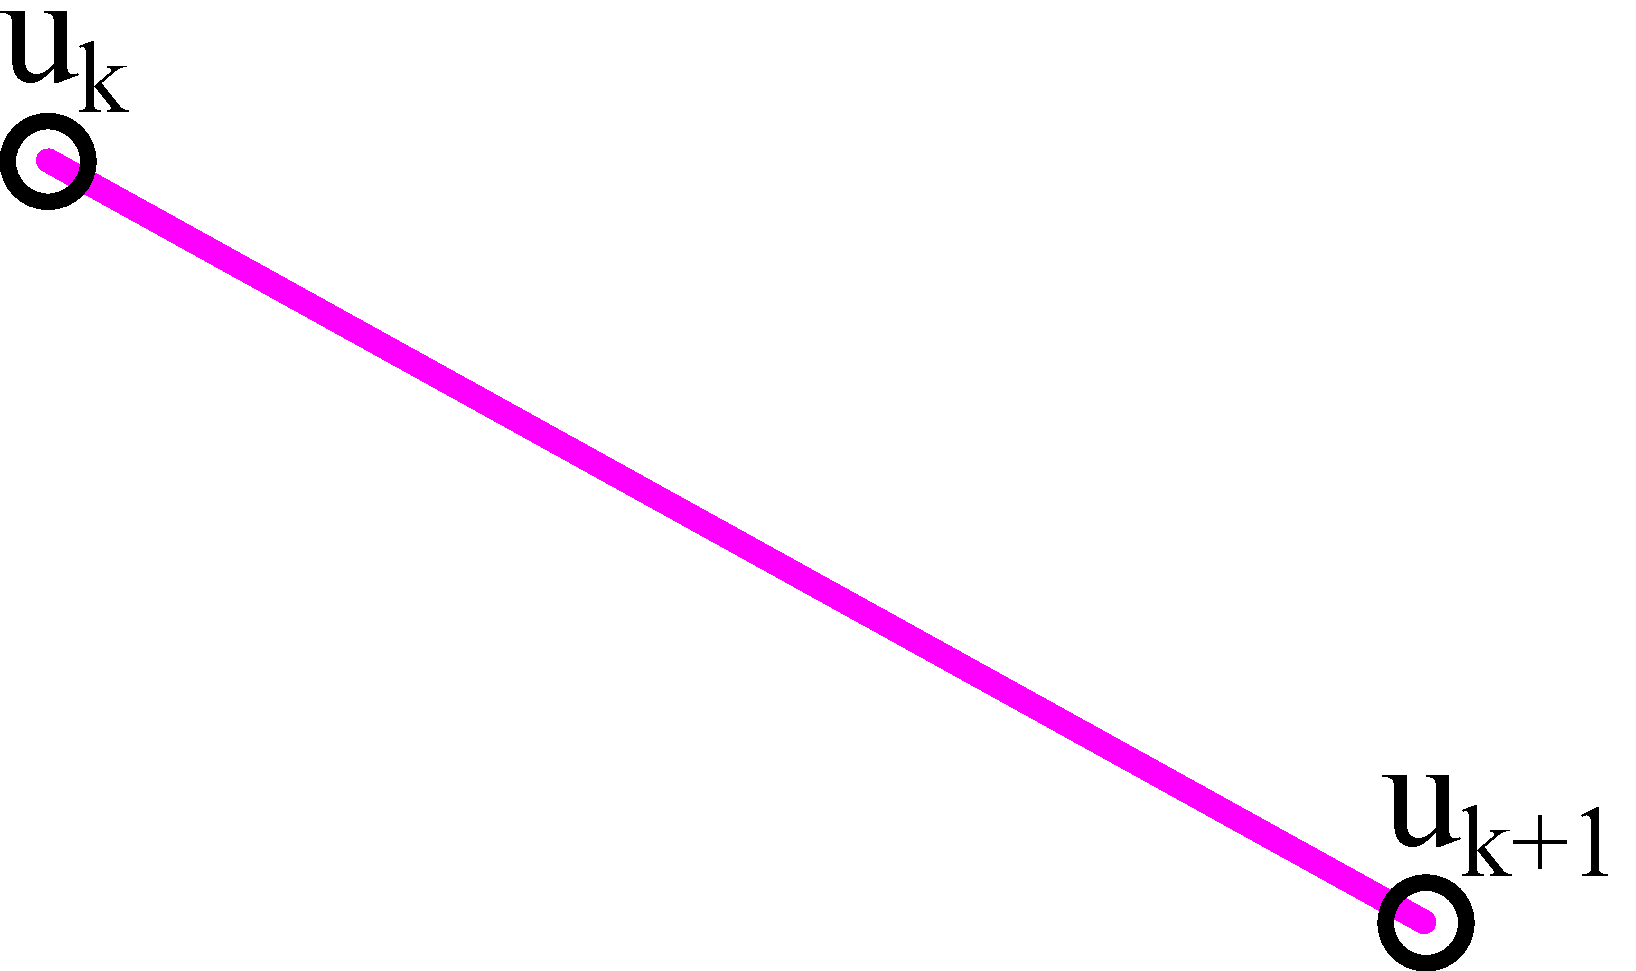
\includegraphics[width=0.7\textwidth]{Cap2/linear-spline.pdf}
        \caption{\textit{Spline} linear de controle}
    \end{subfigure}
    \hfill
    \begin{subfigure}{0.48\linewidth}
        \centering
        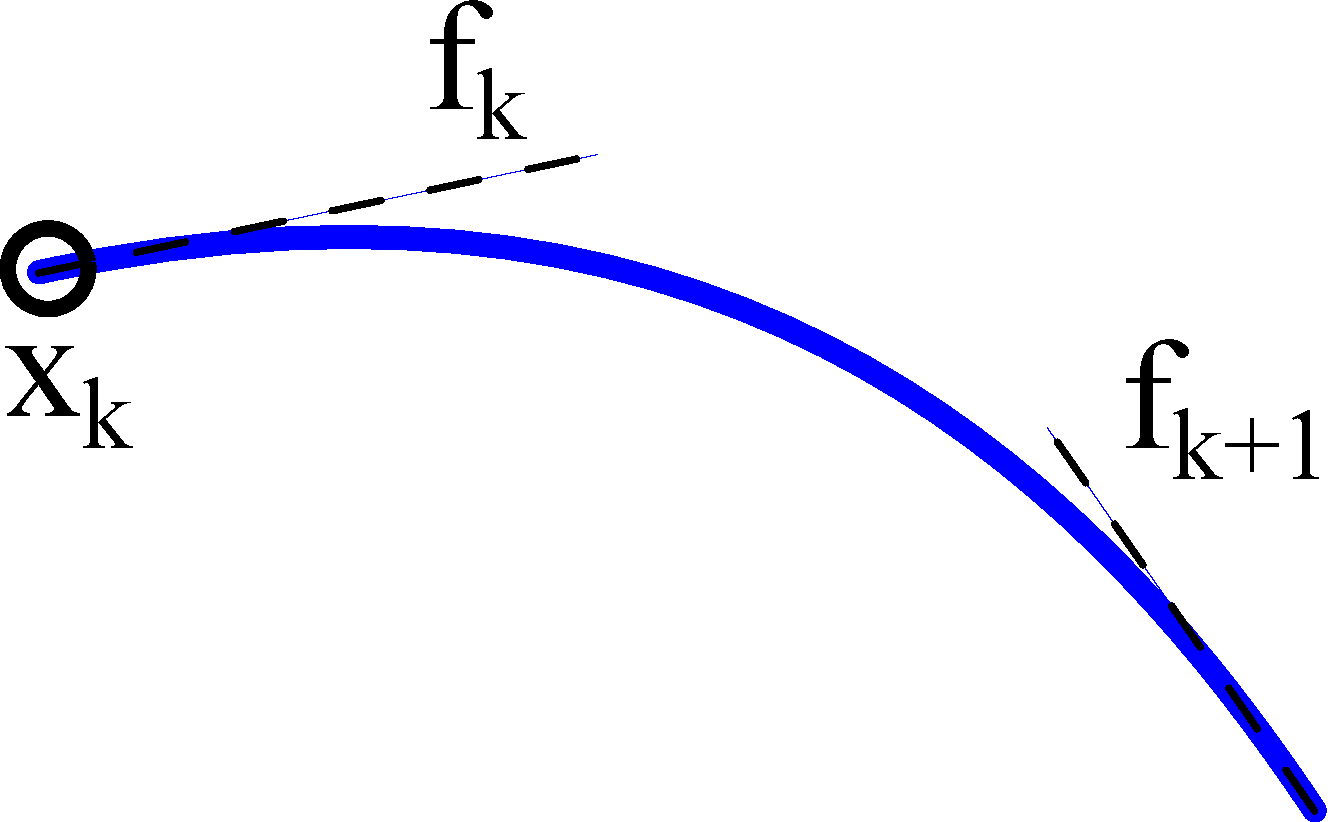
\includegraphics[width=0.57\textwidth]{Cap2/quadratic-spline.pdf}
        \caption{\textit{Spline} quadrática de estado}
    \end{subfigure}
    % \includegraphics[width=0.8\textwidth]{Cap2/}
    \caption{Representações das \textit{splines} de controle e de estado}
    \label{fig:splines}
\end{figure}

Desse modo, as variáveis são definidas como

\begin{equation}
    \mathbf{z}^\intercal = \left( \mathbf{x}_1, \mathbf{u}_1, \cdots, \mathbf{x}_M, \mathbf{u}_M \right),
    \label{eq:z}
\end{equation}

\noindent e as restrições

\begin{equation}
    \boldsymbol{\zeta}_k = \mathbf{x}_{k+1} - \mathbf{x}_k - \dfrac{h_k}{2} \left( \mathbf{f}_{k+1} + \mathbf{f}_k \right),
    \label{eq:defects}
\end{equation}

Assim, pode-se reescrever o índice de desempenho - equação \ref{eq:J} - como

\begin{equation}
    J = \varphi \left[ \mathbf{x} \left( t_0 \right), \mathbf{x} \left( t_f \right), \mathbf{p}, t_0, t_f \right]
    + \sum_{k=0}^{M-1} \dfrac{1}{2} h_k \left( L_{k+1} + L_k \right),
    \label{eq:J-trapezoidal}
\end{equation}




\chapter{Metodologia}
\label{cap:metodologia}

Relembrando, o objetivo deste trabalho é criar uma biblioteca no MATLAB que permita a resolução de problemas de otimização de trajetória de maneira facilitada, de forma que o usuário precise apenas modelar o problema, sem a necessidade de implementar a lógica da solução numérica. Para isso, é necessário que a biblioteca forneça uma interface de dados, de modo a permitir que o usuário entre com a modelagem do seu problema. Além disso, deve-se implementar a colocação trapezoidal como método de solução.

Para validação da implementação a ser realizada, foram implementadas as soluções para alguns problemas exemplos. Tais problemas incluem o estudo de otimização de trajetória de um movimento simples em uma dimensão e braquistócrona, que são problemas clássicos na literatura de otimização de trajetórias, e o estudo de otimização de trajetória de subida de eVTOL em \cite{costa_otimizacao_2023}, o qual utiliza o software PSOPT citado na Seção \ref{sec:rev-bibliografica}.

\section{Interface de Dados}
\label{sec:interface-dados}

Diferente dos softwares OptimTraj \cite{kelly_optimtraj_2022} e PSOPT \cite{becerra_psopt_2022}, a implementação será realizada utilizando uma abordagem de POO, com uma classe MATLAB principal que conterá métodos para a configuração do problema e cálculo da solução. Além da classe principal, a biblioteca contará com funções auxiliares para cálculo da colocação trapezoidal e manipulação de dados.

Os arquivos da biblioteca, assim como os exemplos de uso, estão disponíveis no repositório \cite{simplicio_hsimpliciotg-ita_2024}, e serão descritos na sequência. Para maior clareza, inicialmente será apresentada a classe principal, de modo que será possível entender a estrutura de dados e a lógica de funcionamento da biblioteca. Em seguida, serão apresentadas as funções auxiliares.

\subsection{\texttt{TrajectoryProblem.m}}
\label{subsec:classe-trajectoryproblem}

A classe \texttt{TrajectoryProblem} é a classe principal da biblioteca, e contém métodos para a configuração do problema e cálculo da solução. A classe conta com um construtor, que inicializa os parâmetros e variáveis necessárias para a resolução do problema com valores padrão, e métodos para a configuração dos limites e objetivo do problema, além de um método para a solução numérica do problema.

Dentre os métodos disponíveis, alguns são obrigatórios, ou seja, são necessários para a resolução de qualquer problema, e outros são opcionais, podendo ser utilizados ou não dependendo da necessidade do problema em questão, como pode ser visto na Figura \ref{fig:trajectoryproblem-methods}.

\begin{figure}[H]
    \centering
    \begin{subfigure}{0.6\linewidth}
    \centering
        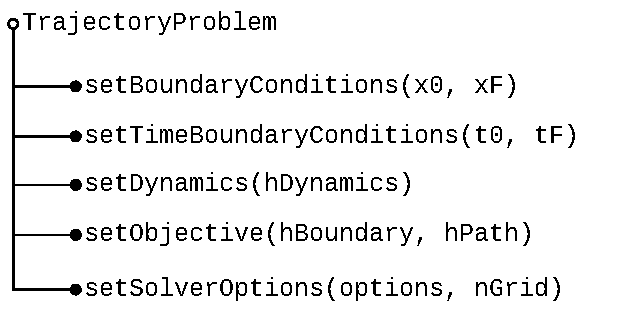
\includegraphics[width=\textwidth]{Cap3/figuras/TrajectoryProblem-mandatory.pdf}
        \caption{Métodos obrigatórios}
    \end{subfigure}
    \hfill
    \begin{subfigure}{0.7\linewidth}
    \centering
        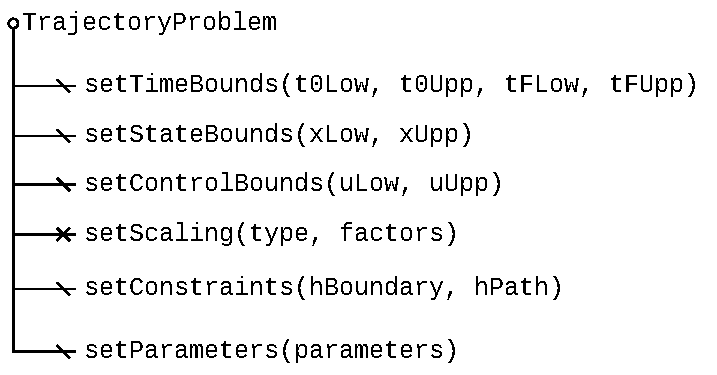
\includegraphics[width=\textwidth]{Cap3/figuras/TrajectoryProblem-optional.pdf}
        \caption{Métodos opcionais}
    \end{subfigure}
    \caption{Métodos da classe \texttt{TrajectoryProblem}}
    \label{fig:trajectoryproblem-methods}
\end{figure}

Além disso, há também métodos auxiliares para a verificação e validação do problema, assim como métodos privados, utilizados internamente pela classe, como pode ser visto na Figura \ref{fig:trajectoryproblem-auxiliar}.

\begin{figure}[H]
    \centering
    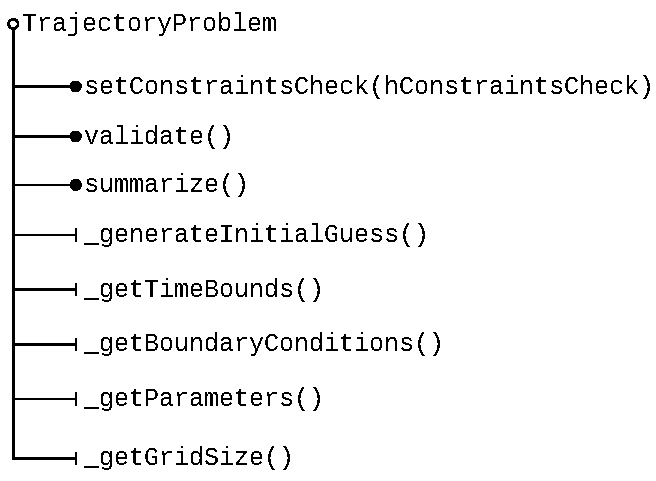
\includegraphics[width=0.64\textwidth]{Cap3/figuras/TrajectoryProblem-auxiliar.pdf}
    \caption{Métodos auxiliares da classe \texttt{TrajectoryProblem}}
    \label{fig:trajectoryproblem-auxiliar}
\end{figure}

Por fim, há o método para a solução do problema com a colocação trapezoidal, apresentado na Figura \ref{fig:trajectoryproblem-solve}, o qual retorna um \texttt{array} de \texttt{structures}, com a solução do problema obtida em cada iteração, além de informações adicionais relacionadas a elas, como apresentado na Figura \ref{fig:solution}.

\begin{figure}[H]
    \centering
    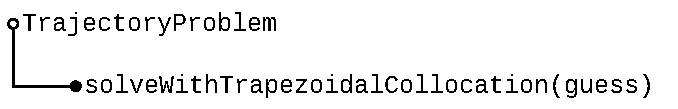
\includegraphics[width=0.66\textwidth]{Cap3/figuras/TrajectoryProblem-solve.pdf}
    \caption{Método para a solução do \texttt{TrajectoryProblem} com a colocação trapezoidal}
    \label{fig:trajectoryproblem-solve}
\end{figure}

\begin{figure}[H]
    \centering
    \begin{subfigure}{0.49\linewidth}
    \centering
        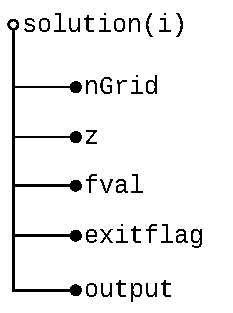
\includegraphics[width=0.45\textwidth]{Cap3/figuras/TrajectoryProblem-solution.pdf}
    \end{subfigure}
    \hfill
    \begin{subfigure}{0.49\linewidth}
    \centering
        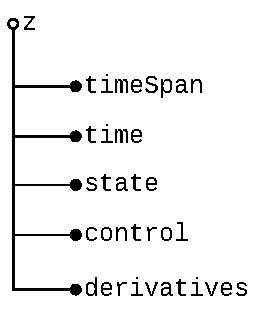
\includegraphics[width=0.52\textwidth]{Cap3/figuras/TrajectoryProblem-solution-z.pdf}
    \end{subfigure}
    \caption{Formato da \texttt{structure} \texttt{solution}}
    \label{fig:solution}
\end{figure}

Na sequência, serão apresentados os métodos da classe, descrevendo sua funcionalidade e uso. O código fonte pode ser encontrado no anexo \ref{sec:codigo-trajectoryproblem}.

\subsubsection{\texttt{.setBoundaryConditions(x0, xF)}}
\label{subsubsec:setboundaryconditions}

Este método recebe como argumentos as condições de contorno do estado do problema, passadas como vetores coluna, os valida e os atribui às propriedades \texttt{x0} e \texttt{xF} da classe.


\subsubsection{\texttt{.setTimeBoundaryConditions(t0, tF)}}
\label{subsubsec:settimeboundaryconditions}

Este método recebe como argumentos os limites de tempo do problema, passados como escalares, os valida e os atribui às propriedades \texttt{t0} e \texttt{tF} da classe.

\subsubsection{\texttt{.setTimeBounds(t0Low, t0Upp, tFLow, tFUpp)}}
\label{subsubsec:settimebounds}

Este método recebe como argumentos os limites de tempo do problema, passados como escalares, os valida e os atribui às propriedades \texttt{t0Low}, \texttt{t0Upp}, \texttt{tFLow} e \texttt{tFUpp} da classe.

\subsubsection{\texttt{.setStateBounds(xLow, xUpp)}}
\label{subsubsec:setstatebounds}

Este método recebe como argumentos os limites de estado do problema, passados como vetores coluna, os valida e os atribui às propriedades \texttt{xLow} e \texttt{xUpp} da classe.

\subsubsection{\texttt{.setControlBounds(uLow, uUpp)}}
\label{subsubsec:setcontrolbounds}

Este método recebe como argumentos os limites de controle do problema, passados como vetores coluna, os valida e os atribui às propriedades \texttt{uLow} e \texttt{uUpp} da classe.

\subsubsection{\texttt{.setScaling(type, factors)}}
\label{subsubsec:setscaling}

Este método recebe como argumentos o tipo de variável a ser escalonada e os fatores de escalonamento, passados como vetores coluna, os valida e os atribui às propriedades \texttt{stateScaling}, \texttt{controlScaling} e \texttt{timeScaling} da classe.

\subsubsection{\texttt{.setDynamics(hDynamics)}}
\label{subsubsec:setdynamics}

Este método recebe como argumento uma função \texttt{handle} que representa a dinâmica do sistema, a qual deve ser definida pelo usuário, a valida e a atribui à propriedade \texttt{dynamics} da classe.


\subsubsection{\texttt{.setObjective(hBoundaryObjective, hPathObjective)}}
\label{subsubsec:setobjective}

Este método recebe como argumento duas funções \texttt{handle} que representam os dois termos da função objetivo do problema, o termo de contorno (Mayer) e o termo de caminho (Lagrange) conforme explicado na Seção \ref{subsec:problema-1}. Tais funções devem ser definidas pelo usuário e serão validadas e atribuídas à propriedade \texttt{objective} da classe, por meio da função \texttt{evaluateObjective}, descrita na Seção \ref{subsec:evaluateobjective}.

\subsubsection{\texttt{.setConstraints(hBoundaryConstraints, hPathConstraints)}}
\label{subsubsec:setconstraints}

Este método recebe como argumento duas funções \texttt{handle} que representam as restrições do problema. Tais funções devem ser definidas pelo usuário e serão validadas e atribuídas à propriedade \texttt{constraints} da classe, por meio da função \texttt{evaluateConstraints}, descrita na Seção \ref{subsec:evaluateconstraints}.

\subsubsection{\texttt{.setParameters(parameters)}}
\label{subsubsec:setparameters}

Este método recebe como argumento um vetor coluna de parâmetros do problema e os atribui à propriedade \texttt{parameters} da classe.

\subsubsection{\texttt{.setVariableNames(stateNames, controlNames)}}
\label{subsubsec:setvariablenames}

Este método recebe como argumento os nomes das variáveis de estado e de controle do problema, passados como vetores de células, e os atribui às propriedades \texttt{stateNames} e \texttt{controlNames} da classe.

\subsubsection{\texttt{.setSolverOptions(options, nGrid)}}
\label{subsubsec:setsolveroptions}

Este método recebe como argumento as opções de solução do problema, passadas como uma \texttt{optimoptions('fmincon')} ou uma célula de tais opções, e o número de pontos de colocação da malha trapezoidal, e os atribui às propriedades \texttt{solverOptions} e \texttt{nGrid} da classe. Caso o argumento seja uma célula, o número de elementos da célula deve ser igual ao número de iterações que serão realizadas. Caso o argumento seja uma única opção de solução, ela será replicada para todas as iterações.

\subsubsection{\texttt{.setConstraintsCheck(hConstraintsCheck)}}
\label{subsubsec:setconstraintscheck}

Este método recebe como argumento uma função \texttt{handle} que representa a função de verificação de restrições do problema, a qual deve ser definida pelo usuário, a valida e a atribui à propriedade \texttt{constraintsCheck} da classe.

\subsubsection{\texttt{.validate()}}
\label{subsubsec:validate}

Este método verifica se todas as propriedades da classe foram definidas, retornando \texttt{true} caso todas as propriedades tenham sido definidas e \texttt{false} caso contrário. Além disso, caso alguma propriedade não tenha sido definida, é exibida uma mensagem de aviso detalhando quais propriedades estão faltando.

\subsubsection{\texttt{.summarize()}}
\label{subsubsec:summarize}

Este método retorna um \texttt{struct} com um resumo das propriedades da classe.

\subsubsection{\texttt{.generateInitialGuess()}}
\label{subsubsec:generateinitialguess}

Este método gera uma estimativa inicial para o problema, retornando um \texttt{struct} com os valores das variáveis de estado e de controle no instante inicial e final, além de uma malha de tempo. Os estados são interpolados linearmente entre os pontos inicial e final, enquanto os controles são considerados constantes e nulos.

\subsubsection{\texttt{.solveWithTrapezoidalCollocation(guess)}}
\label{subsubsec:solvewithtrapezoidalcollocation}

Este método resolve o problema com a colocação trapezoidal, recebendo como argumento uma estimativa inicial para o problema, e retornando um \texttt{array} de \texttt{structures}, com a solução do problema obtida em cada iteração, além de informações adicionais relacionadas a elas, como apresentado na Figura \ref{fig:solution}. Caso o argumento seja omitido, a estimativa inicial é gerada pelo método \texttt{.generateInitialGuess()}.

A partir da primeira iteração, a estimativa inicial é obtida por interpolação dos resultados da iteração anterior, utilizando a função \texttt{spline2} descrita na Seção \ref{subsec:spline2}.

Na chamada do solver \texttt{fmincon}, é interessante notar que, além da função objetivo, da estimativa inicial e das restrições não-lineares, são passadas as restrições inferiores e superiores, que utilizam os limites inferiores e superiores, respectivamente, do tempo inicial e final, dos estados e controles, multiplicados pelos fatores de escalonamento.

\subsubsection{\texttt{.getTimeBounds()}}
\label{subsubsec:gettimebounds}

Este método retorna os limites de tempo do problema.

\subsubsection{\texttt{.getBoundaryConditions()}}
\label{subsubsec:getboundaryconditions}

Este método retorna as condições de contorno do problema.

\subsubsection{\texttt{.getParameters()}}
\label{subsubsec:getparameters}

Este método retorna os parâmetros do problema.

\subsubsection{\texttt{.getGridSize()}}
\label{subsubsec:getgridsize}

Este método retorna o número de pontos de colocação da malha trapezoidal.

\subsection{\texttt{packZ.m}}
\label{subsec:packz}

Esta função recebe como argumentos um intervalo de tempo, a matriz de estado, a matriz de controle e os fatores de escalonamento, e realiza o empacotamento dessas variáveis de decisão em um único vetor. A função também retorna uma \texttt{struct} com informações sobre o empacotamento, de modo que seja possível desempacotar as variáveis de decisão posteriormente.

Tal função é necessária para a inclusão dos tempos inicial e final como variáveis de decisão do problema. Uma opção mais simples seria incluir o vetor de tempos na matriz com os estados e controles, porém, como os tempos intermediários são bem definidos para dados intervalos de tempo e número de pontos de colocação, isso apenas incrementaria a quantidade de variáveis passadas ao solver, sem adicionar informações extras.

\subsection{\texttt{unpackZ.m}}
\label{subsec:unpackz}

Esta função recebe como argumentos o vetor de variáveis de decisão do problema, a \texttt{struct} com informações sobre o empacotamento e uma \texttt{flag} indicando se as variáveis devem ser desescalonadas. A função retorna os valores das variáveis de estado e de controle, desempacotados e eventualmente desescalonados, e o vetor de tempos.

\subsection{\texttt{computeDefects.m}}
\label{subsec:computedefects}

Esta função recebe como argumentos o intervalo de tempo, a matriz de estado e a matriz de derivadas de estado, e retorna a matriz de defeitos da colocação trapezoidal. A matriz de defeitos é calculada utilizando a Equação \ref{eq:defects}, conforme descrito na Seção \ref{subsec:colocacao-trapezoidal}.

\subsection{\texttt{evaluateConstraints.m}}
\label{subsec:evaluateconstraints}

Esta função recebe como argumentos o vetor de variáveis de decisão do problema, a \texttt{struct} com informações sobre o empacotamento, a função \texttt{handle} que define a dinâmica do sistema, as funções \texttt{handle} de restrições de defeitos, de restrições de caminho e de restrições de contorno, e retorna dois vetores de restrições não lineares, de desigualdade e de igualdade.

Inicialmente desempacotam-se os valores das variáveis de decisão, obtendo-se o tempo, o estado e o controle, escalonados e não escalonados. As últimas serão utilizadas para o cálculo das derivadas de estado, que devem grandezas físicas. Em seguida, calcula-se as derivadas de estado, escala-se e calcula-se os defeitos. Por fim, avaliam-se as restrições de defeitos, de caminho e de contorno, retornando os vetores de restrições de desigualdade e de igualdade.

\subsection{\texttt{evaluateObjective.m}}
\label{subsec:evaluateobjective}

Esta função recebe como argumentos o vetor de variáveis de decisão do problema, a \texttt{struct} com informações sobre o empacotamento, as funções \texttt{handle} de termo de contorno e de termo de caminho da função objetivo, e retorna o valor da função objetivo.

Inicialmente desempacotam-se os valores das variáveis de decisão, obtendo-se o tempo, o estado e o controle. Em seguida, avaliam-se os termos de contorno e de caminho da função objetivo, retornando o seu valor final. Ressalta-se a utilização da função \texttt{trapz} para a integração numérica do termo de caminho, conforme Equação \ref{eq:J-trapezoidal}.

\subsection{\texttt{spline2.m}}
\label{subsec:spline2}

Esta função recebe como argumentos o vetor de tempos antigo, a matriz de estados antiga, a matriz de derivadas de estado antigas e o vetor de tempos novo, e retorna a matriz de estados e a matriz de derivadas de estado interpolados e avaliados no tempo novo.

A função utiliza um \textit{loop} para calcular os valores interpolados um por vez. Dentro do \textit{loop}, primeiramente encontra-se o intervalo de tempo no qual o tempo de interesse se encontra, utilizando a função \texttt{find} para localizar o índice do primeiro elemento maior ou igual ao tempo de interesse. Caso o tempo de interesse seja menor que o tempo inicial, o primeiro intervalo é utilizado. Caso o tempo de interesse seja maior que o tempo final, o último intervalo é utilizado.

Em seguida, calcula-se o passo de tempo local, dado pela diferença entre o tempo final e o tempo inicial do intervalo, e, utilizando o index encontrado previamente, obtém-se os valores das variáveis de estado e de suas derivadas no intervalo. Por fim, utiliza-se a fórmula de interpolação de segundo grau, conforme Equação \ref{eq:spline-quadratica}, para realizar a interpolação dos valores das variáveis de estado.

\section{Problemas Exemplos}
\label{sec:problemas-exemplos}

Nesta seção, descrevem-se três problemas exemplo de aplicação da biblioteca desenvolvida. Em ordem crescente de complexidade, são apresentados um problema de minimização de tempo de percurso de uma partícula em uma dimensão na Seção \ref{subsec:movimento-simples}, um problema clássico de otimização, o problema da braquistócrona, na Seção \ref{subsec:braquistocrona}, e um problema de minimização de consumo energético de um veículo multirrotor, na Seção \ref{subsec:evtol}.

Além disso, para não poluir a leitura com a os códigos usados em cada problema, apresenta-se um modelo de utilização da biblioteca, descrito na Seção \ref{subsec:modelo-utilizacao}.

\subsection{Modelo de utilização}
\label{subsec:modelo-utilizacao}

A seguir, apresenta-se um modelo de utilização da biblioteca, que pode ser adaptado para a resolução de outros problemas, alterando-se apenas as funções de dinâmica, objetivo e restrições. Exemplos de implementação de cada uma dessas funções são apresentados no Anexo \ref{sec:arquivos-modelo}.

\begin{code}
    \inputminted[
        frame=leftline,
        framesep=3mm,
        baselinestretch=1.2,
        % breaklines,
        % bgcolor=dracula_bg,
        % rulecolor=dracula_rule,
        bgcolor=light_bg,
        rulecolor=light_rule,
        linenos
    ]{matlab}{Cap3/codigos/modelo_implementacao.m}
    \caption{Modelo de implementação}
    \label{code:modelo-implementacao}
\end{code}


\subsection{Movimento simples em uma dimensão}
\label{subsec:movimento-simples}

Considere um ponto material de massa $m$ que se move sobre uma linha reta, sujeito a uma força $\mathbf{F}$, conforme ilustrado na Figura \ref{fig:movimento-simples}. O problema é modelado utilizando-se a posição e velocidade da partícula como variáveis de estado e a força como variável de controle. O vetor estado, o vetor controle e a dinâmica do sistema são descritos pela Equação \ref{eq:movimento-simples}.

Por fim, o problema consiste em encontrar a trajetória que minimiza o quadrado da força no percurso entre dois pontos - Equação \ref{eq:movimento-simples-J}.

\begin{figure}[H]
    \centering
    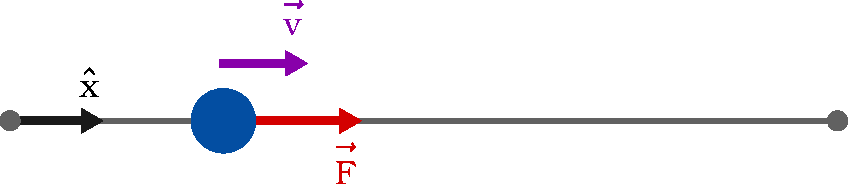
\includegraphics[width=0.72\textwidth]{Cap3/figuras/movimento-simples.pdf}
    \caption{Diagrama de forças no movimento simples}
    \label{fig:movimento-simples}
\end{figure}

\begin{equation}
    \mathbf{x} = \begin{bmatrix}
        s_x \\
        v_x
    \end{bmatrix},
    \qquad
    \mathbf{u} = \begin{bmatrix}
        F
    \end{bmatrix},
    \qquad
    \dot{\mathbf{x}} = \begin{bmatrix}
        v \\
        F/m
    \end{bmatrix},
    \label{eq:movimento-simples}
\end{equation}

\begin{equation}
    J = \int_{t_0}^{t_f} \left[ F^2 \right] dt.
    \label{eq:movimento-simples-J}
\end{equation}

\subsection{Braquistócrona}
\label{subsec:braquistocrona}

O problema da braquistócrona, proposto por Johann Bernoulli em 1696, consiste em encontrar a curva que minimiza o tempo de descida de uma partícula entre dois pontos sob ação da gravidade, desconsiderando o atrito. O nome vem do grego ``\textit{brachistos}'' (mais curto) e ``\textit{chronos}'' (tempo).

Embora possa parecer intuitivo que a linha reta seria a solução ótima por ser o caminho mais curto entre dois pontos, a solução do problema é uma curva cicloide. Isso ocorre porque, apesar do caminho ser mais longo, a partícula consegue atingir velocidades maiores ao longo da trajetória devido à maior inclinação inicial, resultando em um tempo total menor.

Este problema é considerado um dos marcos históricos do cálculo variacional e da otimização de trajetória, tendo sido resolvido por grandes matemáticos como Newton, Leibniz e o próprio Bernoulli. Sua solução analítica pode ser obtida através do princípio de Hamilton, mas aqui será utilizada uma abordagem numérica através da colocação trapezoidal.

Para modelizar o problema, considere um ponto material de massa $m$ sob ação da gravidade, que se move entre dois pontos fixos, conforme ilustrado na Figura \ref{fig:braquistocrona}. Apesar de sabermos que se trata de uma descida, a figura ilustra o ponto final com posições positivas ($s_x,f > 0$ e $s_y,f > 0$), de modo que o ângulo de inclinação da trajetória seja positivo e que se evitem problemas com convenções de sinais.

Utilizam-se as posições horizontal e vertical da partícula, além do valor absoluto da velocidade, como variáveis de estado e o ângulo de inclinação da trajetória como variável de controle. O vetor estado, o vetor controle e a dinâmica do sistema são descritos pelas Equações \ref{eq:braquistocrona}.

Por fim, o problema consiste em encontrar a trajetória que minimiza o tempo de descida entre dois pontos, conforme Equação \ref{eq:braquistocrona-J}.

\begin{figure}[H]
    \centering
    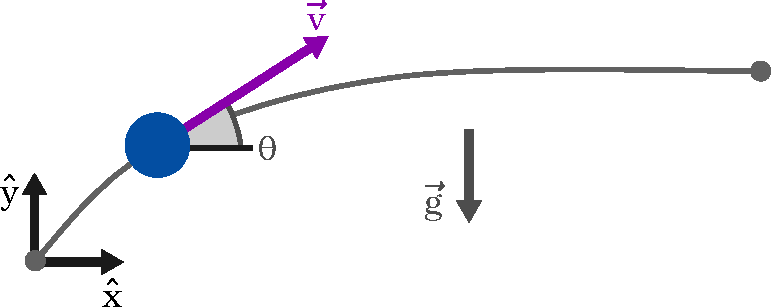
\includegraphics[width=0.72\textwidth]{Cap3/figuras/brachistochrone.pdf}
    \caption{Diagrama de forças no braquistócrona}
    \label{fig:braquistocrona}
\end{figure}

\begin{equation}
    \mathbf{x} = \begin{bmatrix}
        s_x \\
        s_y \\
        v
    \end{bmatrix},
    \qquad
    \mathbf{u} = \begin{bmatrix}
        \theta
    \end{bmatrix},
    \qquad
    \dot{\mathbf{x}} = \begin{bmatrix}
        v \cos(\theta) \\
        v \sin(\theta) \\
        -g \sin(\theta)
    \end{bmatrix},
    \label{eq:braquistocrona}
\end{equation}

\begin{equation}
    J = t_f.
    \label{eq:braquistocrona-J}
\end{equation}


\subsection{Trajetória de subida de eVTOL}
\label{subsec:evtol}

Por fim, apresenta-se o problema descrito em \cite{costa_otimizacao_2023}, que consiste em encontrar a trajetória de subida que minimize o consumo energético de um veículo multirrotor. Para modelar o problema, as variáveis de decisão utilizadas foram as posições $[s_x, s_y]$, velocidades $[v_x, v_y]$, energia total da bateria utilizada $E$ e comandos de tração dos rotores $[T_x, T_y]$, descritos pelas Equações \ref{eq:evtol}.

\begin{equation}
    \mathbf{x} = \begin{bmatrix}
        s_x \\
        s_y \\
        v_x \\
        v_y \\
        E
    \end{bmatrix},
    \qquad
    \mathbf{u} = \begin{bmatrix}
        T_x \\
        T_y
    \end{bmatrix},
    \label{eq:evtol}
\end{equation}

\begin{figure}[H]
    \centering
    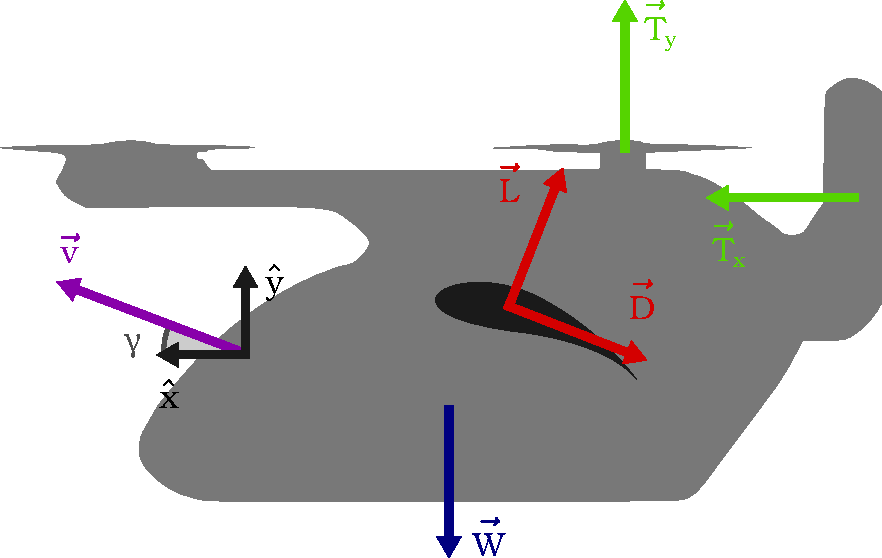
\includegraphics[width=0.72\textwidth]{Cap3/figuras/eVTOL.pdf}
    \caption{Diagrama de forças no eVTOL}
    \label{fig:evtol-forças}
\end{figure}

Conforme a Figura \ref{fig:evtol-forças}, a dinâmica do sistema pode ser descrita pelas Equações \ref{eq:evtol-dinamica}.

\begin{equation}
\begin{aligned}
    m\ddot{p}_x &= F_x = T_x - D(\mathbf{v}) \cos(\gamma) - L(\mathbf{v}) \sin(\gamma) \\
    m\ddot{p}_y &= F_y = T_y - D(\mathbf{v}) \sin(\gamma) + L(\mathbf{v}) \cos(\gamma) - mg,
\end{aligned}
\label{eq:evtol-dinamica}
\end{equation}

\noindent de modo que as restrições diferenciais escrevem-se

\begin{equation}
\begin{aligned}
    \dot{s}_x &= v_x \\
    \dot{s}_y &= v_y \\
    \dot{v}_x &= \dfrac{1}{m} F_x \\
    \dot{v}_y &= \dfrac{1}{m} F_y,
\end{aligned},
\qquad
\begin{aligned}
    \dot{E}
    &= P_{total} \\
    &=
    \begin{aligned}
        &\left( 2 P_{ind,rotor,x} (1 + \chi) + T_x |\mathbf{v}| \cos(-\gamma) \right) \\
        &+ \left( 4 P_{ind,rotor,y} (1 + \chi) + T_y |\mathbf{v}| \sin(-\gamma) \right).
    \end{aligned}
\end{aligned}
\label{eq:evtol-restricoes-diferenciais}
\end{equation}


Para finalizar a formulação do PCO, dado que se almeja o consumo mínimo da bateria, define-se a função objetivo como

\begin{equation}
    J = E_f.
    \label{eq:evtol-J}
\end{equation}



% \chapter{Conclusão}
% \label{cap:conclusão}
% Neste capítulo, são apresentados os resultados obtidos através da aplicação da biblioteca desenvolvida aos problemas-exemplo descritos no Capítulo \ref{cap:metodologia}. Para cada problema, são mostrados os gráficos das trajetórias encontradas, bem como a evolução temporal das variáveis de estado e controle. Além disso, são feitas análises comparativas com resultados da literatura, quando disponíveis, e discussões sobre a qualidade das soluções obtidas.

A apresentação dos resultados está organizada na mesma ordem dos problemas-exemplo: inicialmente, são mostrados os resultados do problema de movimento simples em uma dimensão na Seção \ref{subsec:movimento-simples}; em seguida, os resultados do problema da braquistócrona na Seção \ref{subsec:braquistocrona}; e, por fim, os resultados do problema de trajetória do eVTOL na Seção \ref{subsec:evtol}. Para cada problema, são também discutidos aspectos específicos da implementação e eventuais desafios encontrados durante o processo de otimização.

\section{Movimento simples em uma dimensão}
\label{sec:resultados-movimento-simples}

Como parâmetros para a resolução deste problema, utilizou-se $m=1 \, \si{\kilo\gram}$, $s_{x,0}=0 \, \si{\meter}$, $s_{x,f}=1 \, \si{\meter}$, $t_0=0 \, \si{\second}$ e $t_f=1 \, \si{\second}$. Como chute inicial, interpolou-se linearmente os valores iniciais e finais das variáveis de estado e entre os valores $1 \, \si{\newton}$ e $-1 \, \si{\newton}$ para a variável de controle, como mostrado na Figura \ref{fig:resultados-movimento-simples-chute}.

\begin{figure}
    \centering
    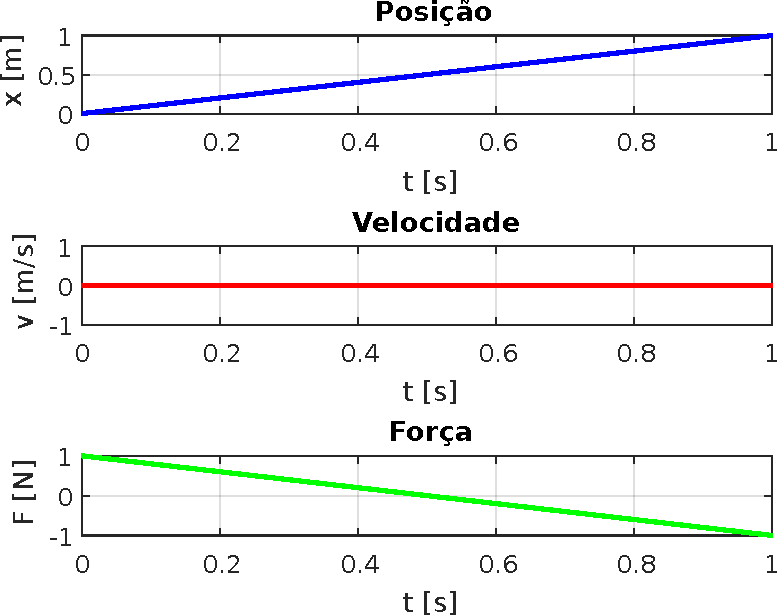
\includegraphics[width=0.65\textwidth]{Cap4/figuras/movimento-simples-chute.pdf}
    \caption{Chute inicial para o problema de movimento simples em uma dimensão.}
    \label{fig:resultados-movimento-simples-chute}
\end{figure}

Como opções do solver, foram utilizados $n=30$ pontos de colocação, sem necessidade de refinamento da malha e nem de ajustes extras de parâmetros para que houvesse convergência para a solução ótima. O resultado é apresentado na Figura \ref{fig:resultados-movimento-simples}.

\begin{figure}[H]
    \centering
    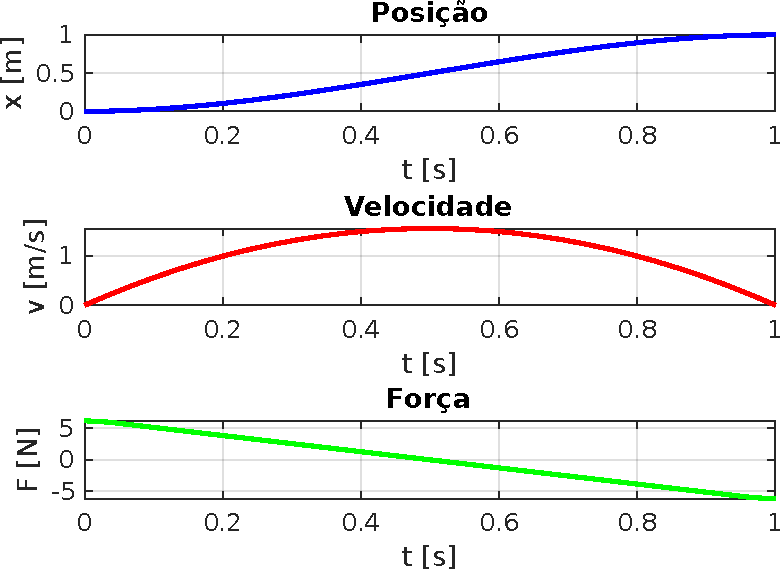
\includegraphics[width=0.65\textwidth]{Cap4/figuras/movimento-simples.pdf}
    \caption{Trajetória ótima do problema de movimento simples em uma dimensão.}
    \label{fig:resultados-movimento-simples}
\end{figure}


\section{Pêndulo invertido}
\label{sec:resultados-pendulo-invertido}

Para a resolução deste problema, utilizou-se $m=1 \, \si{\kilo\gram}$, $l=0,5 \, \si{\meter}$, $b=0,1 \, \si{\newton\second\per\meter}$ e $g=9,81 \, \si{\meter\per\second\squared}$ como parâmetros. Não foi necessário utilizar um chute inicial elaborado, uma vez que o solver encontrou a solução ótima sem dificuldades.

Como opções do solver, utilizou-se uma sequência de refinamento da malha, com $n=[30, 60]$ pontos de colocação. Além disso, apenas aumentou-se o número máximo de avaliações da função por iteração para que o solver convergisse para a solução ótima. O resultado é apresentado na Figura \ref{fig:resultados-pendulo-invertido}.

\begin{figure}[H]
    \centering
    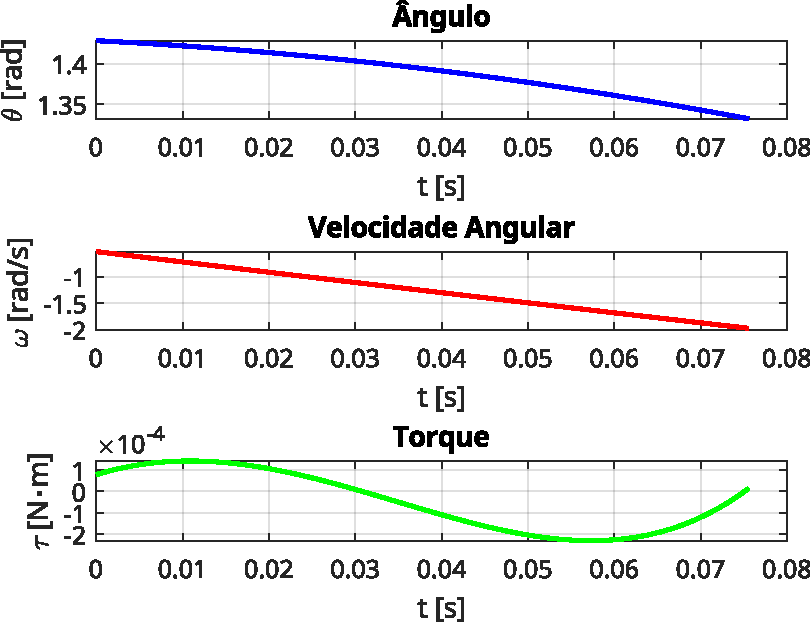
\includegraphics[width=0.65\textwidth]{Cap4/figuras/pendulo-invertido.pdf}
    \caption{Trajetória ótima do problema de pêndulo invertido.}
    \label{fig:resultados-pendulo-invertido}
\end{figure}

\section{Manobra de mudança de faixa}
\label{sec:resultados-manobra-mudanca-faixa}

Como parâmetros para a resolução deste problema, utilizou-se $a_{max}=2 \, \si{\meter\per\second\squared}$, $v_{alvo}=15 \, \si{\meter\per\second}$, $w_{faixa}=3,5 \, \si{\meter}$ e $x_f=75 \, \si{\meter}$ como parâmetros. Também não foi necessário utilizar um chute inicial elaborado, uma vez que o solver encontrou a solução ótima sem dificuldades.

Como opções do solver, utilizou-se uma sequência de refinamento da malha, com $n=[20, 40, 80]$ pontos de colocação. Além disso, assim como no problema do pêndulo invertido, apenas ajustou-se o número máximo de avaliações da função por iteração para que o solver convergisse para a solução ótima. O resultado é apresentado na Figura \ref{fig:resultados-manobra-mudanca-faixa}.

\begin{figure}[H]
    \centering
    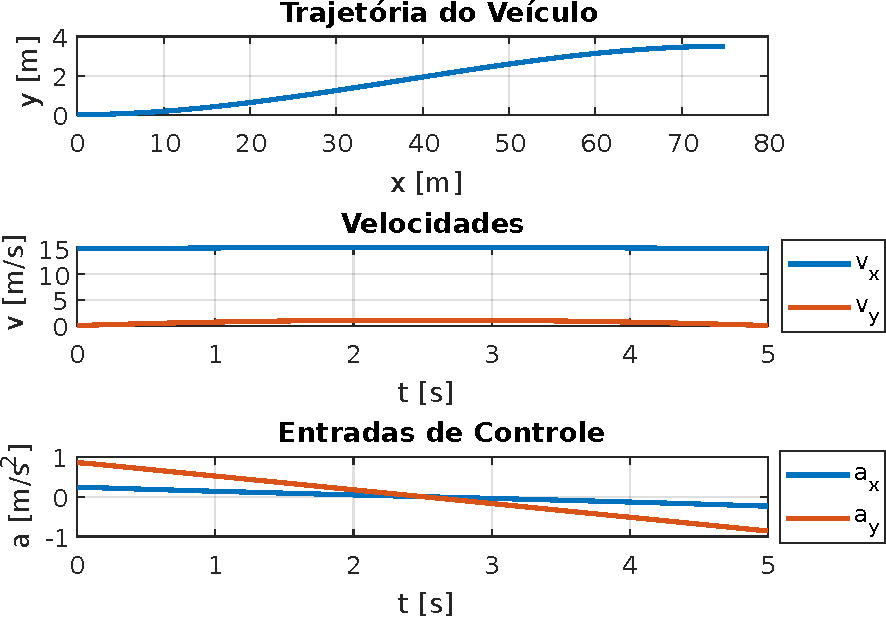
\includegraphics[width=0.77\textwidth]{Cap4/figuras/manobra-mudanca-faixa.pdf}
    \caption{Trajetória ótima do problema de manobra de mudança de faixa.}
    \label{fig:resultados-manobra-mudanca-faixa}
\end{figure}

\section{Braquistócrona}
\label{sec:resultados-braquistocrona}

Para a resolução deste problema, utilizou-se $m=1 \, \si{\kilo\gram}$, $s_{0}=(0,0) \, \si{\meter}$, $s_{f}=(5,-5) \, \si{\meter}$ e $v_0=0 \, \si{\meter\per\second}$ como parâmetros. Como chute inicial, utilizou-se uma parábola horizontal, como mostrado na Figura \ref{fig:resultados-braquistocrona-chute}.

\begin{figure}[H]
    \centering
    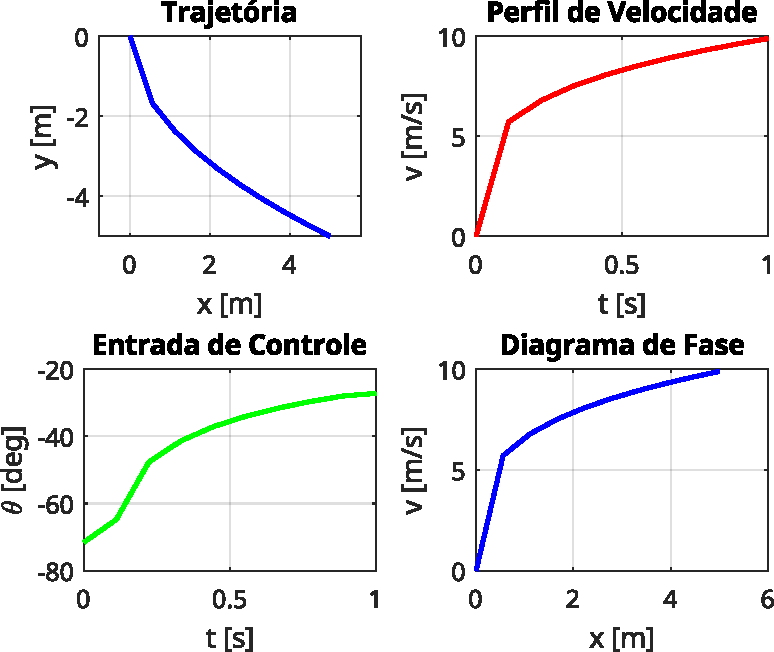
\includegraphics[width=0.68\textwidth]{Cap4/figuras/braquistocrona-chute.pdf}
    \caption{Chute inicial para o problema de braquistócrona.}
    \label{fig:resultados-braquistocrona-chute}
\end{figure}

Como opções do solver, foi utilizada uma sequência de refinamento da malha, com $n=[10, 20, 40]$ pontos de colocação. Além disso, foram utilizadas diversas outras opções de parâmetros para que o solver convergisse para a solução ótima, como o uso de um algoritmo de otimização mais robusto e uma tolerância para a verificação de restrições mais restritiva. Apesar dos esforços, o solver não convergiu para a solução ótima na última iteração, de modo que não se encontrou a solução ótima. Ainda assim, encontrou-se um resultado factível, o qual é apresentado na Figura \ref{fig:resultados-braquistocrona}.

\begin{figure}[H]
    \centering
    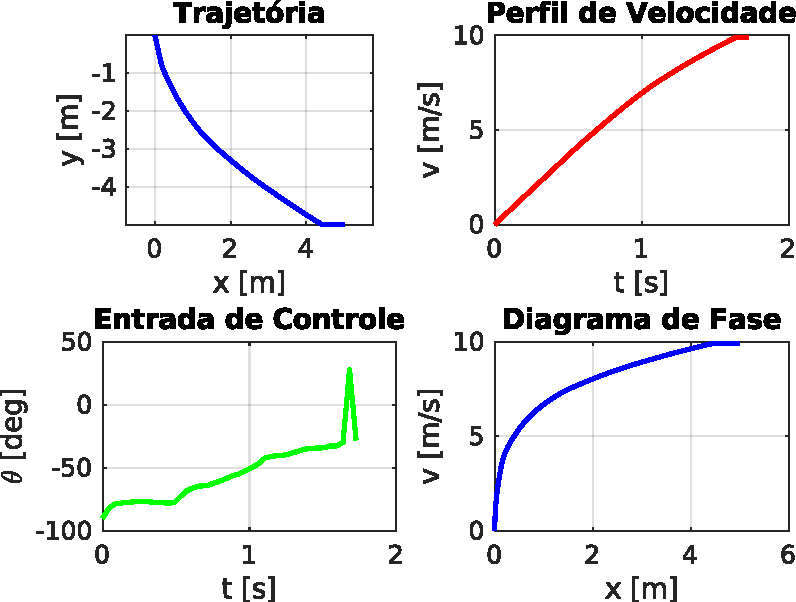
\includegraphics[width=0.7\textwidth]{Cap4/figuras/braquistocrona.pdf}
    \caption{Trajetória ótima do problema de braquistócrona.}
    \label{fig:resultados-braquistocrona}
\end{figure}

Na Figura \ref{fig:resultados-braquistocrona-comparacao} é apresentada a comparação entre a solução obtida e a solução analítica do problema, a qual é uma ciclóide.

\begin{figure}[H]
    \centering
    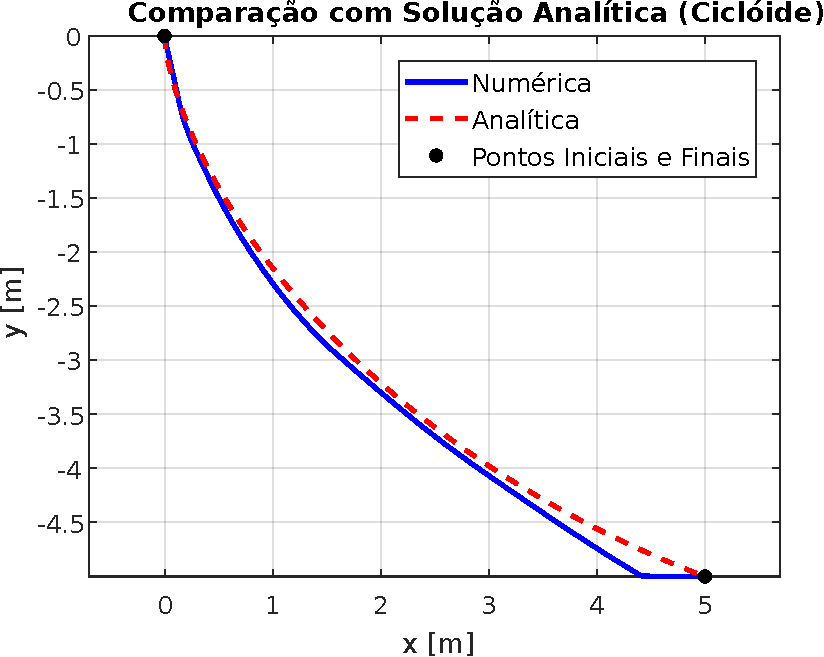
\includegraphics[width=0.65\textwidth]{Cap4/figuras/braquistocrona-comparacao.pdf}
    \caption{Comparação entre a solução obtida e a solução analítica.}
    \label{fig:resultados-braquistocrona-comparacao}
\end{figure}


\section{Trajetória do eVTOL}
\label{sec:resultados-evtol}

O problema considerado é o caso base do trabalho de referência, utilizando-se os mesmos parâmetros nele apresentados. Testou-se também a utilização do mesmo chute inicial, mas sem sucesso. Desse modo, construiu-se um chute inicial fisicamente plausível utilizando-se um polinômio de terceiro grau para a trajetória e respeitando as relações entre as variáveis de estado e controle, como mostrado na Figura \ref{fig:resultados-evtol-chute}.

\begin{figure}[H]
    \centering
    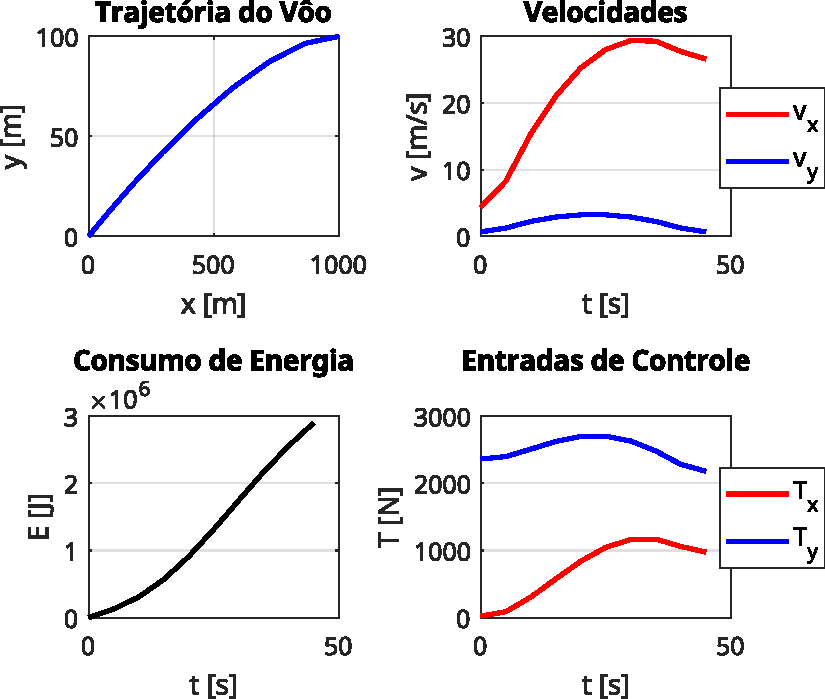
\includegraphics[width=0.75\textwidth]{Cap4/figuras/evtol-chute.pdf}
    \caption{Chute inicial para o problema de trajetória do eVTOL.}
    \label{fig:resultados-evtol-chute}
\end{figure}

Como opções do solver, utilizou-se uma sequência de refinamento da malha, com $n=[10, 20, 40, 80]$ pontos de colocação. Além disso, assim como no problema da braquistócrona, foram utilizadas diversas outras opções de parâmetros para que o solver convergisse para a solução ótima, como o uso de um algoritmo de otimização mais robusto e uma tolerância para a verificação de restrições mais restritiva.

Apesar dos esforços, o solver não encontrou um ótimo local nem mesmo nas iterações com menos pontos na malha. O melhor resultado obtido é apresentado na Figura \ref{fig:resultados-evtol}.

\begin{figure}[H]
    \centering
    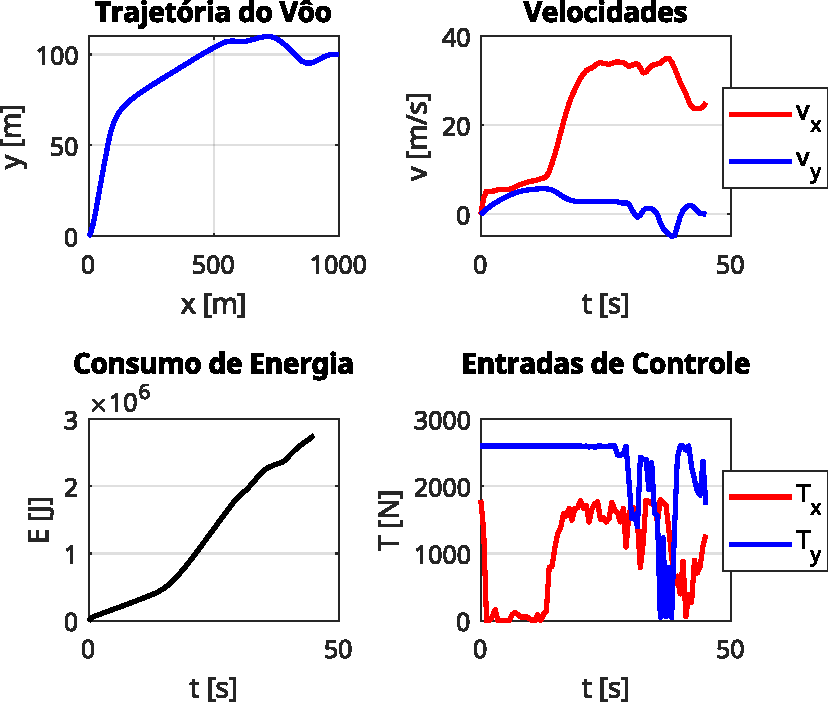
\includegraphics[width=0.75\textwidth]{Cap4/figuras/evtol.pdf}
    \caption{Trajetória ótima do problema de trajetória do eVTOL.}
    \label{fig:resultados-evtol}
\end{figure}

Apesar da solução não ser a ótima e as entradas de controle não serem suaves, a trajetória encontrada é fisicamente plausível e o consumo de energia é menor do que o da solução de referência, sendo $E=2,75484 \, \si{\mega\joule}$ para a solução obtida comparado a $E=2,94342 \, \si{\mega\joule}$ da referência. A Figura \ref{fig:resultados-evtol-comparacao} mostra a comparação entre a solução obtida e a solução de referência.

\begin{figure}[H]
    \centering
    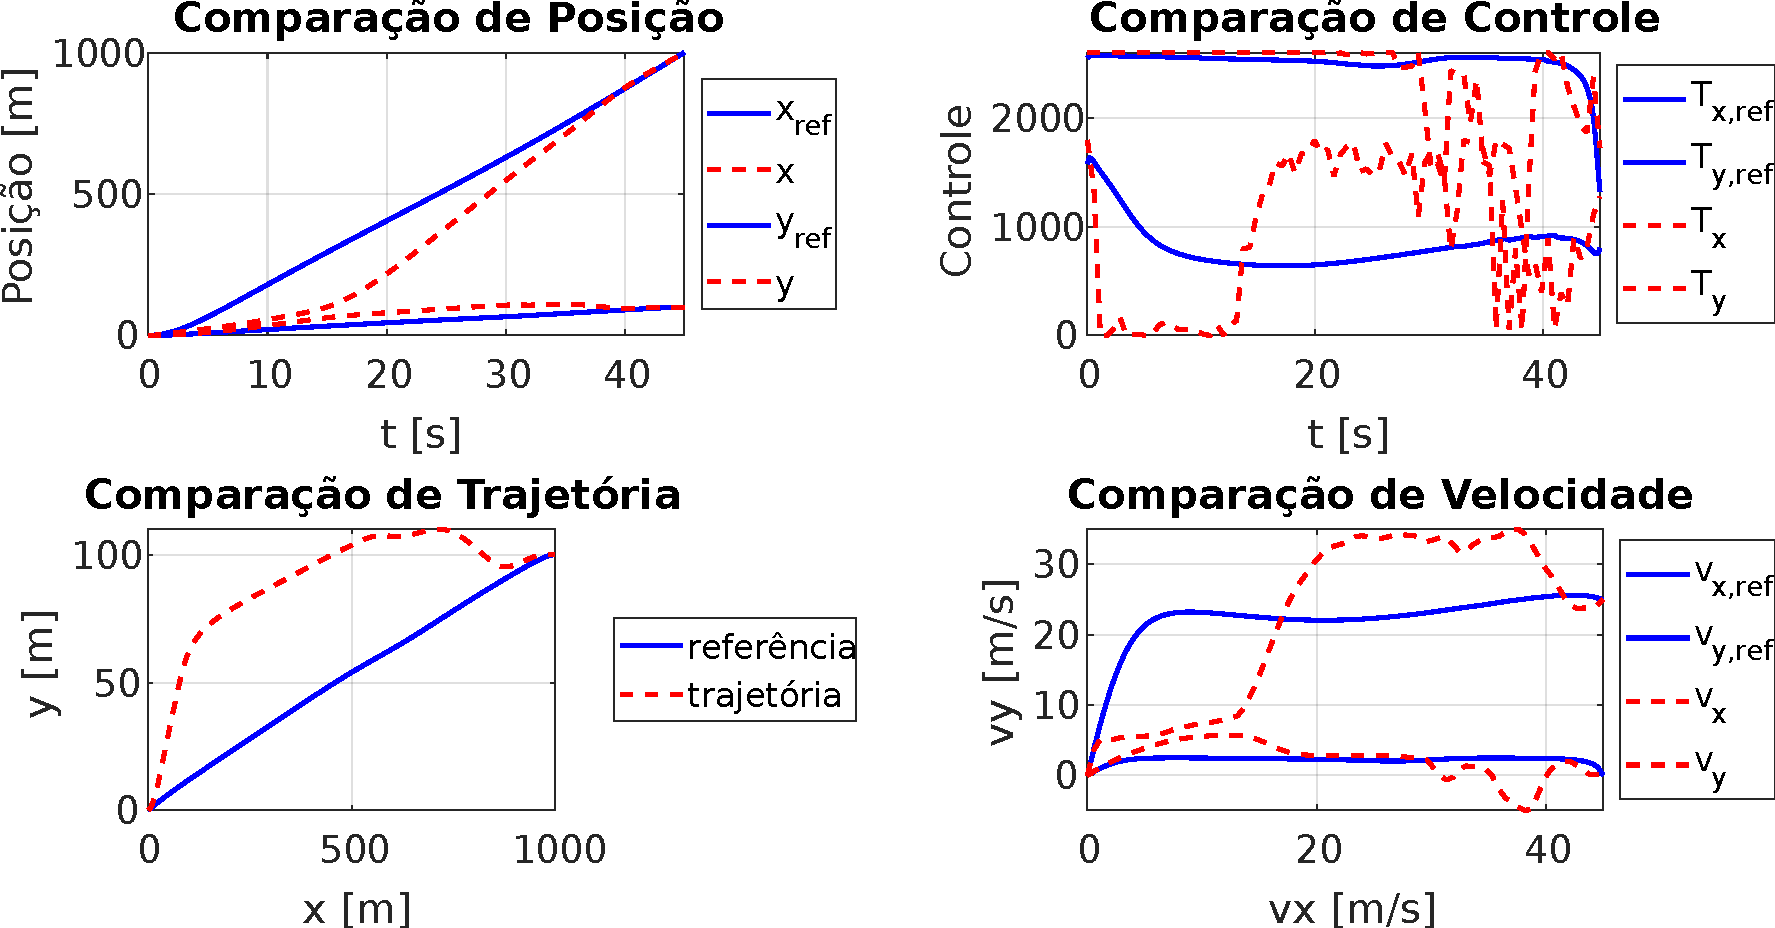
\includegraphics[width=\textwidth]{Cap4/figuras/evtol-comparacao.pdf}
    \caption{Comparação entre a solução obtida e a solução de referência.}
    \label{fig:resultados-evtol-comparacao}
\end{figure}

\begin{figure}[H]
    \centering
    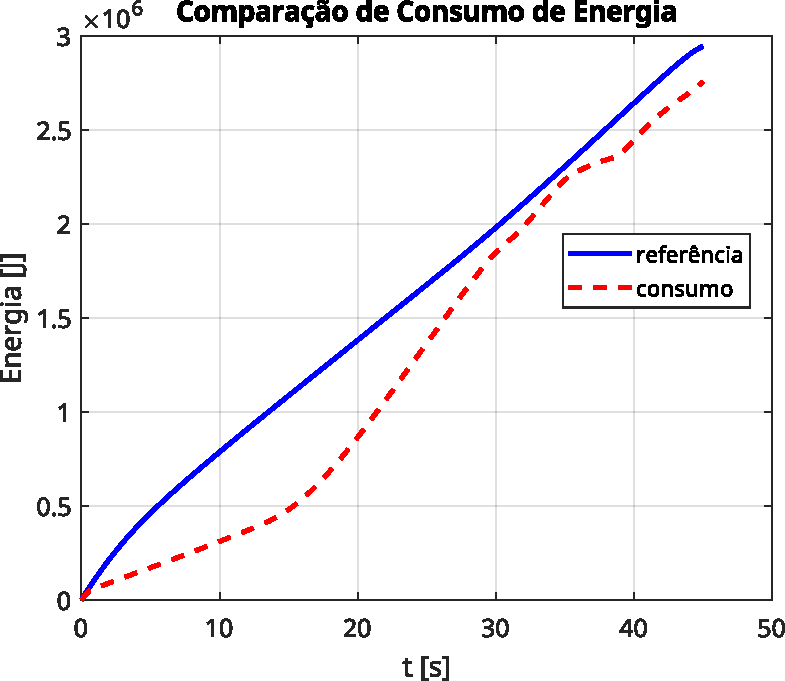
\includegraphics[width=0.65\textwidth]{Cap4/figuras/evtol-comparacao-energia.pdf}
    \caption{Comparação da energia.}
    \label{fig:resultados-evtol-comparacao-energia}
\end{figure}


% REFERENCIAS BIBLIOGRAFICAS
\renewcommand\bibname{\itareferencesnamebabel} % renomear título do capítulo referências
\bibliography{Referencias/referencias}

% Apendices
% \appendix
% \chapter{Tópicos de Dilema Linear} % opcional
% \section{Uma Primeira Seção para o Apêndice}

A matriz de Dilema Linear $M$ e o vetor de torques inerciais $b$,
utilizados na simulação são calculados segundo a formulação 
abaixo:
\begin{equation}
M=\left[ \begin{array}{ccc}
M_{11} & M_{12} & M_{13} \\
M_{21} & M_{22} & M_{23} \\
M_{31} & M_{32} & M_{33}
\end{array} \right]
\end{equation}


% Anexos
% \annex
% \chapter{Exemplo de um Primeiro Anexo} % opcional
% Nessa seção, serão apresentados os arquivos de código fonte do projeto. Os mesmo arquivos estão disponíveis no repositório do projeto \cite{simplicio_hsimpliciotg-ita_2024}. Para melhor visualização, sugere-se que o leitor abra os arquivos no editor de sua preferência.

\section{Arquivos da biblioteca}
\label{sec:arquivos-biblioteca}

\subsection{\texttt{TrajectoryProblem.m}}
\label{sec:codigo-trajectoryproblem}

\begin{code}
    \inputminted[
        frame=leftline,
        framesep=3mm,
        baselinestretch=1.2,
        bgcolor=light_bg,
        rulecolor=light_rule,
        linenos
    ]{matlab}{AneA/codigos/TrajectoryProblem.m}
    \caption{Classe \texttt{TrajectoryProblem}}
    \label{code:trajectoryproblem}
\end{code}

\subsection{\texttt{packZ.m}}
\label{sec:codigo-packz}

\begin{code}
    \inputminted[
        frame=leftline,
        framesep=3mm,
        baselinestretch=1.2,
        bgcolor=light_bg,
        rulecolor=light_rule,
        linenos
    ]{matlab}{AneA/codigos/packZ.m}
    \caption{Função \texttt{packZ}}
    \label{code:packz}
\end{code}

\subsection{\texttt{unpackZ.m}}
\label{sec:codigo-unpackz}

\begin{code}
    \inputminted[
        frame=leftline,
        framesep=3mm,
        baselinestretch=1.2,
        bgcolor=light_bg,
        rulecolor=light_rule,
        linenos
    ]{matlab}{AneA/codigos/unpackZ.m}
    \caption{Função \texttt{unpackZ}}
    \label{code:unpackz}
\end{code}

\subsection{\texttt{computeDefects.m}}
\label{sec:codigo-computedefects}

\begin{code}
    \inputminted[
        frame=leftline,
        framesep=3mm,
        baselinestretch=1.2,
        bgcolor=light_bg,
        rulecolor=light_rule,
        linenos
    ]{matlab}{AneA/codigos/computeDefects.m}
    \caption{Função \texttt{computeDefects}}
    \label{code:computedefects}
\end{code}

\subsection{\texttt{evaluateConstraints.m}}
\label{sec:codigo-evaluateconstraints}

\begin{code}
    \inputminted[
        frame=leftline,
        framesep=3mm,
        baselinestretch=1.2,
        bgcolor=light_bg,
        rulecolor=light_rule,
        linenos
    ]{matlab}{AneA/codigos/evaluateConstraints.m}
    \caption{Função \texttt{evaluateConstraints}}
    \label{code:evaluateconstraints}
\end{code}

\subsection{\texttt{evaluateObjective.m}}
\label{sec:codigo-evaluateobjective}

\begin{code}
    \inputminted[
        frame=leftline,
        framesep=3mm,
        baselinestretch=1.2,
        bgcolor=light_bg,
        rulecolor=light_rule,
        linenos
    ]{matlab}{AneA/codigos/evaluateObjective.m}
    \caption{Função \texttt{evaluateObjective}}
    \label{code:evaluateobjective}
\end{code}

\subsection{\texttt{spline2.m}}
\label{sec:codigo-spline2}

\begin{code}
    \inputminted[
        frame=leftline,
        framesep=3mm,
        baselinestretch=1.2,
        bgcolor=light_bg,
        rulecolor=light_rule,
        linenos
    ]{matlab}{AneA/codigos/spline2.m}
    \caption{Função \texttt{spline2}}
    \label{code:spline2}
\end{code}


\section{Arquivos de modelo}
\label{sec:arquivos-modelo}

\subsection{\texttt{mainTemplate.m}}
\label{sec:codigo-maintemplate}

\begin{code}
    \inputminted[
        frame=leftline,
        framesep=3mm,
        baselinestretch=1.2,
        bgcolor=light_bg,
        rulecolor=light_rule,
        linenos
    ]{matlab}{AneA/codigos/template/mainTemplate.m}
    \caption{Arquivo principal do template}
    \label{code:maintemplate}
\end{code}

\subsection{\texttt{templateDynamics.m}}
\label{sec:codigo-templatedynamics}

\begin{code}
    \inputminted[
        frame=leftline,
        framesep=3mm,
        baselinestretch=1.2,
        bgcolor=light_bg,
        rulecolor=light_rule,
        linenos
    ]{matlab}{AneA/codigos/template/templateDynamics.m}
    \caption{Função \texttt{templateDynamics}}
    \label{code:templatedynamics}
\end{code}


\subsection{\texttt{templateParams.m}}
\label{sec:codigo-templateparams}

\begin{code}
    \inputminted[
        frame=leftline,
        framesep=3mm,
        baselinestretch=1.2,
        bgcolor=light_bg,
        rulecolor=light_rule,
        linenos
    ]{matlab}{AneA/codigos/template/templateParams.m}
    \caption{Função \texttt{templateParams}}
    \label{code:templateparams}
\end{code}

\subsection{\texttt{boundaryConstraints.m}}
\label{sec:codigo-boundaryconstraints}

\begin{code}
    \inputminted[
        frame=leftline,
        framesep=3mm,
        baselinestretch=1.2,
        bgcolor=light_bg,
        rulecolor=light_rule,
        linenos
    ]{matlab}{AneA/codigos/template/boundaryConstraints.m}
    \caption{Função \texttt{boundaryConstraints}}
    \label{code:boundaryconstraints}
\end{code}


\subsection{\texttt{pathConstraints.m}}
\label{sec:codigo-pathconstraints}

\begin{code}
    \inputminted[
        frame=leftline,
        framesep=3mm,
        baselinestretch=1.2,
        bgcolor=light_bg,
        rulecolor=light_rule,
        linenos
    ]{matlab}{AneA/codigos/template/pathConstraints.m}
    \caption{Função \texttt{pathConstraints}}
    \label{code:pathconstraints}
\end{code}


\subsection{\texttt{boundaryObjective.m}}
\label{sec:codigo-boundaryobjective}

\begin{code}
    \inputminted[
        frame=leftline,
        framesep=3mm,
        baselinestretch=1.2,
        bgcolor=light_bg,
        rulecolor=light_rule,
        linenos
    ]{matlab}{AneA/codigos/template/boundaryObjective.m}
    \caption{Função \texttt{boundaryObjective}}
    \label{code:boundaryobjective}
\end{code}


\subsection{\texttt{pathObjective.m}}
\label{sec:codigo-pathobjective}

\begin{code}
    \inputminted[
        frame=leftline,
        framesep=3mm,
        baselinestretch=1.2,
        bgcolor=light_bg,
        rulecolor=light_rule,
        linenos
    ]{matlab}{AneA/codigos/template/pathObjective.m}
    \caption{Função \texttt{pathObjective}}
    \label{code:pathobjective}
\end{code}


\section{Arquivos do problema movimento simples}
\label{sec:arquivos-problema-movimento-simples}

\subsection{\texttt{mainSimpleMass.m}}
\label{sec:codigo-mainsimplemass}

\begin{code}
    \inputminted[
        frame=leftline,
        framesep=3mm,
        baselinestretch=1.2,
        bgcolor=light_bg,
        rulecolor=light_rule,
        linenos
    ]{matlab}{AneA/codigos/simple_mass/mainSimpleMass.m}
    \caption{Arquivo principal do problema movimento simples}
    \label{code:mainsimplemass}
\end{code}


\subsection{\texttt{simpleMassDynamics.m}}
\label{sec:codigo-simplemassdynamics}

\begin{code}
    \inputminted[
        frame=leftline,
        framesep=3mm,
        baselinestretch=1.2,
        bgcolor=light_bg,
        rulecolor=light_rule,
        linenos
    ]{matlab}{AneA/codigos/simple_mass/simpleMassDynamics.m}
    \caption{Função \texttt{simpleMassDynamics}}
    \label{code:simplemassdynamics}
\end{code}


\subsection{\texttt{boundaryConstraints.m}}
\label{sec:codigo-boundaryconstraints-simplemass}

\begin{code}
    \inputminted[
        frame=leftline,
        framesep=3mm,
        baselinestretch=1.2,
        bgcolor=light_bg,
        rulecolor=light_rule,
        linenos
    ]{matlab}{AneA/codigos/simple_mass/boundaryConstraints.m}
    \caption{Função \texttt{boundaryConstraints}}
    \label{code:boundaryconstraints-simplemass}
\end{code}


\subsection{\texttt{pathConstraints.m}}
\label{sec:codigo-pathconstraints-simplemass}

\begin{code}
    \inputminted[
        frame=leftline,
        framesep=3mm,
        baselinestretch=1.2,
        bgcolor=light_bg,
        rulecolor=light_rule,
        linenos
    ]{matlab}{AneA/codigos/simple_mass/pathConstraints.m}
    \caption{Função \texttt{pathConstraints}}
    \label{code:pathconstraints-simplemass}
\end{code}


\subsection{\texttt{boundaryObjective.m}}
\label{sec:codigo-boundaryobjective-simplemass}

\begin{code}
    \inputminted[
        frame=leftline,
        framesep=3mm,
        baselinestretch=1.2,
        bgcolor=light_bg,
        rulecolor=light_rule,
        linenos
    ]{matlab}{AneA/codigos/simple_mass/boundaryObjective.m}
    \caption{Função \texttt{boundaryObjective}}
    \label{code:boundaryobjective-simplemass}
\end{code}


\subsection{\texttt{pathObjective.m}}
\label{sec:codigo-pathobjective-simplemass}

\begin{code}
    \inputminted[
        frame=leftline,
        framesep=3mm,
        baselinestretch=1.2,
        bgcolor=light_bg,
        rulecolor=light_rule,
        linenos
    ]{matlab}{AneA/codigos/simple_mass/pathObjective.m}
    \caption{Função \texttt{pathObjective}}
    \label{code:pathobjective-simplemass}
\end{code}


\subsection{\texttt{generateSimpleMassGuess.m}}
\label{sec:codigo-generatesimplemassguess}

\begin{code}
    \inputminted[
        frame=leftline,
        framesep=3mm,
        baselinestretch=1.2,
        bgcolor=light_bg,
        rulecolor=light_rule,
        linenos
    ]{matlab}{AneA/codigos/simple_mass/generateSimpleMassGuess.m}
    \caption{Função \texttt{generateSimpleMassGuess}}
    \label{code:generatesimplemassguess}
\end{code}


\section{Arquivos do problema da braquistócrona}
\label{sec:arquivos-problema-braquistocrona}

\subsection{\texttt{mainBrachistochrone.m}}
\label{sec:codigo-mainbrachistochrone}

\begin{code}
    \inputminted[
        frame=leftline,
        framesep=3mm,
        baselinestretch=1.2,
        bgcolor=light_bg,
        rulecolor=light_rule,
        linenos
    ]{matlab}{AneA/codigos/brachistochrone/mainBrachistochrone.m}
    \caption{Arquivo principal do problema da braquistócrona}
    \label{code:mainbrachistochrone}
\end{code}


\subsection{\texttt{brachistochroneDynamics.m}}
\label{sec:codigo-brachistochronedynamics}

\begin{code}
    \inputminted[
        frame=leftline,
        framesep=3mm,
        baselinestretch=1.2,
        bgcolor=light_bg,
        rulecolor=light_rule,
        linenos
    ]{matlab}{AneA/codigos/brachistochrone/brachistochroneDynamics.m}
    \caption{Função \texttt{brachistochroneDynamics}}
    \label{code:brachistochronedynamics}
\end{code}


\subsection{\texttt{brachistochroneParams.m}}
\label{sec:codigo-brachistochroneparams}

\begin{code}
    \inputminted[
        frame=leftline,
        framesep=3mm,
        baselinestretch=1.2,
        bgcolor=light_bg,
        rulecolor=light_rule,
        linenos
    ]{matlab}{AneA/codigos/brachistochrone/brachistochroneParams.m}
    \caption{Função \texttt{brachistochroneParams}}
    \label{code:brachistochroneparams}
\end{code}


\subsection{\texttt{boundaryConstraints.m}}
\label{sec:codigo-boundaryconstraints-brachistochrone}

\begin{code}
    \inputminted[
        frame=leftline,
        framesep=3mm,
        baselinestretch=1.2,
        bgcolor=light_bg,
        rulecolor=light_rule,
        linenos
    ]{matlab}{AneA/codigos/brachistochrone/boundaryConstraints.m}
    \caption{Função \texttt{boundaryConstraints}}
    \label{code:boundaryconstraints-brachistochrone}
\end{code}


\subsection{\texttt{pathConstraints.m}}
\label{sec:codigo-pathconstraints-brachistochrone}

\begin{code}
    \inputminted[
        frame=leftline,
        framesep=3mm,
        baselinestretch=1.2,
        bgcolor=light_bg,
        rulecolor=light_rule,
        linenos
    ]{matlab}{AneA/codigos/brachistochrone/pathConstraints.m}
    \caption{Função \texttt{pathConstraints}}
    \label{code:pathconstraints-brachistochrone}
\end{code}


\subsection{\texttt{boundaryObjective.m}}
\label{sec:codigo-boundaryobjective-brachistochrone}

\begin{code}
    \inputminted[
        frame=leftline,
        framesep=3mm,
        baselinestretch=1.2,
        bgcolor=light_bg,
        rulecolor=light_rule,
        linenos
    ]{matlab}{AneA/codigos/brachistochrone/boundaryObjective.m}
    \caption{Função \texttt{boundaryObjective}}
    \label{code:boundaryobjective-brachistochrone}
\end{code}


\subsection{\texttt{pathObjective.m}}
\label{sec:codigo-pathobjective-brachistochrone}

\begin{code}
    \inputminted[
        frame=leftline,
        framesep=3mm,
        baselinestretch=1.2,
        bgcolor=light_bg,
        rulecolor=light_rule,
        linenos
    ]{matlab}{AneA/codigos/brachistochrone/pathObjective.m}
    \caption{Função \texttt{pathObjective}}
    \label{code:pathobjective-brachistochrone}
\end{code}


\subsection{\texttt{generateBrachistochroneGuesses.m}}
\label{sec:codigo-generatebrachistochroneguesses}

\begin{code}
    \inputminted[
        frame=leftline,
        framesep=3mm,
        baselinestretch=1.2,
        bgcolor=light_bg,
        rulecolor=light_rule,
        linenos
    ]{matlab}{AneA/codigos/brachistochrone/generateBrachistochroneGuess.m}
    \caption{Função \texttt{generateBrachistochroneGuess}}
    \label{code:generatebrachistochroneguess}
\end{code}


\subsection{\texttt{checkConstraints.m}}
\label{sec:codigo-checkconstraints}

\begin{code}
    \inputminted[
        frame=leftline,
        framesep=3mm,
        baselinestretch=1.2,
        bgcolor=light_bg,
        rulecolor=light_rule,
        linenos
    ]{matlab}{AneA/codigos/brachistochrone/checkConstraints.m}
    \caption{Função \texttt{checkConstraints}}
    \label{code:checkconstraints}
\end{code}


\subsection{\texttt{compareWithAnalytical.m}}
\label{sec:codigo-comparewithanalytical}

\begin{code}
    \inputminted[
        frame=leftline,
        framesep=3mm,
        baselinestretch=1.2,
        bgcolor=light_bg,
        rulecolor=light_rule,
        linenos
    ]{matlab}{AneA/codigos/brachistochrone/compareWithAnalytical.m}
    \caption{Função \texttt{compareWithAnalytical}}
    \label{code:comparewithanalytical}
\end{code}


\section{Arquivos do problema do eVTOL}
\label{sec:arquivos-problema-evtol}

\subsection{\texttt{mainEvtol.m}}
\label{sec:codigo-mainevtol}

\begin{code}
    \inputminted[
        frame=leftline,
        framesep=3mm,
        baselinestretch=1.2,
        bgcolor=light_bg,
        rulecolor=light_rule,
        linenos
    ]{matlab}{AneA/codigos/evtol/mainEvtol.m}
    \caption{Arquivo principal do problema do eVTOL}
    \label{code:mainevtol}
\end{code}


\subsection{\texttt{evtolDynamics.m}}
\label{sec:codigo-evtoldynamics}

\begin{code}
    \inputminted[
        frame=leftline,
        framesep=3mm,
        baselinestretch=1.2,
        bgcolor=light_bg,
        rulecolor=light_rule,
        linenos
    ]{matlab}{AneA/codigos/evtol/evtolDynamics.m}
    \caption{Função \texttt{evtolDynamics}}
    \label{code:evtoldynamics}
\end{code}


\subsection{\texttt{computeLiftDrag.m}}
\label{sec:codigo-computeliftdrag}

\begin{code}
    \inputminted[
        frame=leftline,
        framesep=3mm,
        baselinestretch=1.2,
        bgcolor=light_bg,
        rulecolor=light_rule,
        linenos
    ]{matlab}{AneA/codigos/evtol/computeLiftDrag.m}
    \caption{Função \texttt{computeLiftDrag}}
    \label{code:computeliftdrag}
\end{code}


\subsection{\texttt{computeInducedVelocity.m}}
\label{sec:codigo-computeinducedvelocity}

\begin{code}
    \inputminted[
        frame=leftline,
        framesep=3mm,
        baselinestretch=1.2,
        bgcolor=light_bg,
        rulecolor=light_rule,
        linenos
    ]{matlab}{AneA/codigos/evtol/computeInducedVelocity.m}
    \caption{Função \texttt{computeInducedVelocity}}
    \label{code:computeinducedvelocity}
\end{code}


\subsection{\texttt{computeFlightAngle.m}}
\label{sec:codigo-computeflightangle}

\begin{code}
    \inputminted[
        frame=leftline,
        framesep=3mm,
        baselinestretch=1.2,
        bgcolor=light_bg,
        rulecolor=light_rule,
        linenos
    ]{matlab}{AneA/codigos/evtol/computeFlightAngle.m}
    \caption{Função \texttt{computeFlightAngle}}
    \label{code:computeflightangle}
\end{code}


\subsection{\texttt{evtolParams.m}}
\label{sec:codigo-evtolparams}

\begin{code}
    \inputminted[
        frame=leftline,
        framesep=3mm,
        baselinestretch=1.2,
        bgcolor=light_bg,
        rulecolor=light_rule,
        linenos
    ]{matlab}{AneA/codigos/evtol/evtolParams.m}
    \caption{Função \texttt{evtolParams}}
    \label{code:evtolparams}
\end{code}


\subsection{\texttt{boundaryConstraints.m}}
\label{sec:codigo-boundaryconstraints-evtol}

\begin{code}
    \inputminted[
        frame=leftline,
        framesep=3mm,
        baselinestretch=1.2,
        bgcolor=light_bg,
        rulecolor=light_rule,
        linenos
    ]{matlab}{AneA/codigos/evtol/boundaryConstraints.m}
    \caption{Função \texttt{boundaryConstraints}}
    \label{code:boundaryconstraints-evtol}
\end{code}


\subsection{\texttt{pathConstraints.m}}
\label{sec:codigo-pathconstraints-evtol}

\begin{code}
    \inputminted[
        frame=leftline,
        framesep=3mm,
        baselinestretch=1.2,
        bgcolor=light_bg,
        rulecolor=light_rule,
        linenos
    ]{matlab}{AneA/codigos/evtol/pathConstraints.m}
    \caption{Função \texttt{pathConstraints}}
    \label{code:pathconstraints-evtol}
\end{code}


\subsection{\texttt{boundaryObjective.m}}
\label{sec:codigo-boundaryobjective-evtol}

\begin{code}
    \inputminted[
        frame=leftline,
        framesep=3mm,
        baselinestretch=1.2,
        bgcolor=light_bg,
        rulecolor=light_rule,
        linenos
    ]{matlab}{AneA/codigos/evtol/boundaryObjective.m}
    \caption{Função \texttt{boundaryObjective}}
    \label{code:boundaryobjective-evtol}
\end{code}


\subsection{\texttt{pathObjective.m}}
\label{sec:codigo-pathobjective-evtol}

\begin{code}
    \inputminted[
        frame=leftline,
        framesep=3mm,
        baselinestretch=1.2,
        bgcolor=light_bg,
        rulecolor=light_rule,
        linenos
    ]{matlab}{AneA/codigos/evtol/pathObjective.m}
    \caption{Função \texttt{pathObjective}}
    \label{code:pathobjective-evtol}
\end{code}


\subsection{\texttt{physicalInitialGuess.m}}
\label{sec:codigo-physicalinitialguess}

\begin{code}
    \inputminted[
        frame=leftline,
        framesep=3mm,
        baselinestretch=1.2,
        bgcolor=light_bg,
        rulecolor=light_rule,
        linenos
    ]{matlab}{AneA/codigos/evtol/physicalInitialGuess.m}
    \caption{Função \texttt{physicalInitialGuess}}
    \label{code:physicalinitialguess}
\end{code}


\subsection{\texttt{checkConstraints.m}}
\label{sec:codigo-checkconstraints-evtol}

\begin{code}
    \inputminted[
        frame=leftline,
        framesep=3mm,
        baselinestretch=1.2,
        bgcolor=light_bg,
        rulecolor=light_rule,
        linenos
    ]{matlab}{AneA/codigos/evtol/checkConstraints.m}
    \caption{Função \texttt{checkConstraints}}
    \label{code:checkconstraints-evtol}
\end{code}

\subsection{\texttt{testAeroForces.m}}
\label{sec:codigo-testaeroforces}

\begin{code}
    \inputminted[
        frame=leftline,
        framesep=3mm,
        baselinestretch=1.2,
        bgcolor=light_bg,
        rulecolor=light_rule,
        linenos
    ]{matlab}{AneA/codigos/evtol/testAeroForces.m}
    \caption{Função \texttt{testAeroForces}}
    \label{code:testaeroforces}
\end{code}


\subsection{\texttt{testEvtolDynamics.m}}
\label{sec:codigo-testevtoldynamics}

\begin{code}
    \inputminted[
        frame=leftline,
        framesep=3mm,
        baselinestretch=1.2,
        bgcolor=light_bg,
        rulecolor=light_rule,
        linenos
    ]{matlab}{AneA/codigos/evtol/testEvtolDynamics.m}
    \caption{Função \texttt{testEvtolDynamics}}
    \label{code:testevtoldynamics}
\end{code}



% Glossario
%\itaglossary
%\printglossary

% Folha de Registro do Documento
% Valores dos campos do formulario
\FRDitadata{¿¿ de novembro de 2024}
\FRDitadocnro{DCTA/ITA/DM-¿¿¿/2024} %(o número de registro você solicita a biblioteca)
\FRDitaorgaointerno{Instituto Tecnológico de Aeronáutica -- ITA}
%Exemplo no caso de pós-graduação: Instituto Tecnológico de Aeronáutica -- ITA
\FRDitapalavrasautor{Controle Ótimo; Otimização de Trajetória; Colocação Direta}
\FRDitapalavrasresult{¿; ¿; ¿}
%Exemplo no caso de graduação (TG):
\FRDitapalavraapresentacao{Trabalho de Graduação, ITA, São José dos Campos, 2024. \NumPenultimaPagina\ páginas.}
%Exemplo no caso de pós-graduação (msc, dsc):
% \FRDitapalavraapresentacao{ITA, São José dos Campos. Curso de Mestrado. Programa de Pós-Graduação em Engenharia Aeronáutica e Mecânica. Área de Sistemas Aeroespaciais e Mecatrônica. Orientador: Prof.~Dr. Adalberto Santos Dupont. Coorientadora: Prof$^\textnormal{a}$.~Dr$^\textnormal{a}$. Doralice Serra. Defesa em 05/03/2015. Publicada em 25/03/2015.}
\FRDitaresumo{Este trabalho apresenta o desenvolvimento de uma biblioteca em MATLAB para solução de problemas de otimização de trajetória utilizando o método de colocação direta trapezoidal. A biblioteca visa simplificar a resolução deste tipo de problema, permitindo que o usuário concentre-se apenas na modelagem, sem necessidade de implementar a lógica matemática da solução numérica. A implementação é validada através de três casos de teste: um problema de movimento unidimensional simples, o problema clássico da braquistócrona e um problema de otimização de trajetória de subida de uma aeronave eVTOL. Os resultados obtidos são comparados com soluções analíticas, quando disponíveis, e com resultados da literatura utilizando outros softwares de otimização. O trabalho contribui para a área de controle ótimo ao disponibilizar uma ferramenta que facilita a implementação de soluções numéricas para problemas de otimização de trajetória, sendo particularmente útil para aplicações em engenharia aeroespacial e áreas correlatas.}
%  Primeiro Parametro: Nacional ou Internacional -- N/I
%  Segundo parametro: Ostensivo, Reservado, Confidencial ou Secreto -- O/R/C/S
\FRDitaOpcoes{N}{O}
% Cria o formulario
\itaFRD

\end{document}
% Fim do Documento. O massacre acabou!!! :-)
